\documentclass[11pt]{article}
\usepackage[margin=2.6cm]{geometry}
\usepackage{graphicx,booktabs,amsmath,microtype}
\usepackage{float}   % [H]: figures stay where they are written
\usepackage[hidelinks]{hyperref}
\usepackage[dvipsnames]{xcolor}
\graphicspath{{figures/}}
\newcommand{\code}[1]{\texttt{\small #1}}
\setlength{\parskip}{4pt}\setlength{\parindent}{0pt}
\title{Health measures for the prevention project\\[2pt]
\large Construction, validation, and the choice among them}
\author{Julian Ashwin}
\date{August 2026}

\begin{document}
\maketitle

\noindent Built and validated by \code{data\_cleaning/03--06} and
\code{descriptives/01--07}; every number here is printed by those scripts'
self-validation output. This note records which UKHLS health variables the
project uses, how each measure is constructed and why, what the new
graded-response measures deliver against everything that came before them
(the original physical GRM, PCS/MCS, the physical-only composite, SF-6D,
GHQ), and how the ever-diagnosis, dimensionality and ceiling questions
resolve.

\tableofcontents

\section{The variable inventory}

Measurement models are restricted to items asked in (nearly) every wave, so a
score means the same thing wherever it lands in the panel. Presence was
verified against the raw headers of all fifteen \code{indresp} files, labels
against the UKDA-6614 dictionaries.

\begin{center}\small
\begin{tabular}{p{7.6cm}p{2.4cm}p{4.6cm}}
\toprule
Variables & Waves & Used \\
\midrule
SF-12, all 12 items (self-completion preferred) & all 15 & both GRMs; PCS/MCS rebuild; SF-6D \\
GHQ-12 items (\code{scghqa..l}, 4 categories) & all 15 & mental GRM \\
Impairment list \code{disdif1..12}, gated on \code{health} & all 15 & physical GRM (FUNC testlet) \\
Long-standing illness (\code{health}) & all 15 & gate for \code{disdif}; descriptive \\
Diagnosed conditions (\code{hcond*} families, codes 1--17) & all 15 (\S2) & condition items; sensitivities \\
Health satisfaction (\code{sclfsat1}) & all 15 & validation outcome only \\
SWEMWBS; ADL module; loneliness & 1/4/7/10/13; 7/9/11/13; 9--15 & excluded: fail the every-wave rule \\
Hospital out- and in-patient attendance (\code{hl2gp}, \code{hosp}; \S\ref{sec:convexity} on the absent GP count) & 7--15 & criterion-validity outcomes \\
Height/weight (self-report) & wave 1 only & excluded (biomarkers are UKDA-7251, not held) \\
\bottomrule
\end{tabular}
\end{center}

\section{Chronic conditions}

\subsection{Construction}
UKHLS asks the full ``ever diagnosed'' inventory (\code{hcond1..17}) at a
person's \emph{first} interview; later waves record conditions newly reported
since the last interview under a name that changes with questionnaire
redesigns --- \code{hcondn\{i\}} in waves 2--9; from the wave-10 redesign,
\code{hcondcode\{i\}} and \code{hcondncode\{i\}}, both present in waves
10--15 and both used --- all dictionary-verified. The
running indicator (\emph{ever had condition $i$ by wave $w$ $\Leftrightarrow$
reported in any family at any wave $\le w$}) is monotone and defined from the
first inventory onward (76\% of person-waves). Only the wave-1 code list is
used, so the definition is identical in every wave. Per-condition indicators,
diagnosis ages and group counts live in
\code{chronic\_conditions.parquet}; nothing is collapsed before modelling.

This corrects two defects in the earlier EIT count, which used
\code{hcondns*} (``still has \emph{newly diagnosed} condition'') as its
new-report family: that family has no codes 6 and 7 at all --- every
in-panel heart attack and stroke was missed --- and it drops new diagnoses
reported as already resolved. Our count is $\ge$ the EIT count on
100.000\% of 458k person-waves (exact on 94.2\%; 26{,}516 documented
additions, concentrated in MI, stroke and cancer).

\subsection{Why ``ever'', not ``current''}
The ``still has'' family (\code{hconds\#\#}) is asked \emph{only at the wave
a condition is reported}: at wave 6, of 5{,}090 ever-asthma respondents,
$\sim$570 were routed to it. A per-wave ``current'' variable would be
$\sim$90\% carry-forward imputation. Beyond measurability, self-reported
remission conflates control with cure --- managed hypertension and diabetes
read as ``no longer have'', the mechanism behind the under-reporting found
against measured disease (Johnston, Propper \& Shields 2009) and GP records
(Kriegsman et al.\ 1996: good agreement for diabetes, poor for heart disease
and arthritis). The monotone ever-indicator matches the deficit-accumulation
tradition (Mitnitski, Mogilner \& Rockwood 2001; Searle et al.\ 2008). Its
genuine cost --- old diagnoses shadowing current health --- is quantified in
\S\ref{sec:ever}, not assumed away.

\subsection{Why grouped, not seventeen indicators}
\label{sec:groups}
Grouping is the testlet logic applied to diagnoses. CHD, angina, MI, CHF and
stroke are one disease process reported several ways; as separate items they
would violate local independence exactly as the \code{sf2a}/\code{sf2b} pair
did before the original GRM collapsed them (Wainer \& Kiely 1987; Yen 1993).
Rare conditions (1--2\% prevalence) also make weak, unstable IRT items ---
minimum prevalence is an explicit deficit-inclusion criterion in Searle et
al.\ (2008) --- and groups keep a stable clinical meaning while the code list
grows (cf.\ Barnett et al.\ 2012). An ordinal within-group count (0/1/2+)
keeps a severity gradient the way $\mathrm{PF}=\code{sf2a}+\code{sf2b}$ does.
The groupings follow the disease process rather than the questionnaire.
\textbf{CVD} collects the several names UKHLS gives to one underlying
process --- atherosclerosis and its consequences --- which is why a
respondent can plausibly report three of its five items at once.
\textbf{METAB} keeps the two long-term managed conditions apart from those
acute events: hypertension and diabetes are treated rather than survived, and
both are far commoner. \textbf{RESP} spans the chronic airway diseases;
\textbf{MSK} is the single commonest cause of physical limitation in the
data; \textbf{CANCER} stays alone because it is a distinct process and the
one most relevant to mortality. \textbf{OTHER} pools the remainder, none of
which reaches 5\%, so that no item has to be estimated on a prevalence near
1\%.

The seventeen conditions, their groups, and what each one is:

\begin{center}\small
\begin{tabular}{llp{6.5cm}r}
\toprule
Group & Condition & What it is & Ever \\
\midrule
\textbf{CVD} & angina & chest pain when the heart's blood supply cannot meet demand, typically on exertion & 2.9\% \\
 & heart attack & a blocked artery kills part of the heart muscle & 2.7\% \\
 & coronary heart disease & the arteries feeding the heart narrow with fatty deposits & 2.4\% \\
 & stroke & blood supply to part of the brain is cut off, damaging brain tissue & 2.1\% \\
 & congestive heart failure & the heart pumps too weakly, causing breathlessness and fluid retention & 0.8\% \\
 & \emph{any of the above} & & \emph{7.4\%} \\
\addlinespace
\textbf{METAB} & high blood pressure & blood pressure persistently above the healthy range & 21.4\% \\
 & diabetes & the body cannot regulate blood sugar properly & 7.2\% \\
 & \emph{either} & & \emph{24.7\%} \\
\addlinespace
\textbf{RESP} & asthma & airways narrow and inflame in episodes, causing wheeze and breathlessness & 15.4\% \\
 & chronic bronchitis & long-term airway inflammation with persistent cough and phlegm & 2.0\% \\
 & emphysema & the lungs' air sacs are permanently damaged, so breathing is laboured & 0.8\% \\
 & \emph{any of the above} & & \emph{16.7\%} \\
\addlinespace
\textbf{MSK} & arthritis & painful inflammation and stiffness of the joints & 16.2\% \\
\addlinespace
\textbf{CANCER} & cancer or malignancy & any malignant tumour & 5.1\% \\
\addlinespace
\textbf{OTHER} & hypothyroidism & an under-active thyroid gland, slowing the body's metabolism & 4.2\% \\
 & liver condition & any long-term liver disease, such as cirrhosis or hepatitis & 2.2\% \\
 & hyperthyroidism & an over-active thyroid gland, speeding the metabolism up & 1.3\% \\
 & epilepsy & a tendency to recurrent seizures from abnormal electrical activity in the brain & 1.3\% \\
 & \emph{any of the above} & & \emph{8.1\%} \\
\addlinespace
\textbf{DEPR}$^{\dagger}$ & clinical depression & a diagnosed depressive disorder, as distinct from transient low mood & 8.2\% \\
\bottomrule
\end{tabular}

{\scriptsize ``Ever'' is the share of person-waves at which the condition has
been reported at or before that wave, among the 458{,}468 person-waves with
an inventory. Conditions are listed within group by prevalence.
$^{\dagger}$DEPR is the one group assigned to the mental bank rather than the
physical one.}
\end{center}

\subsection{Diagnosis timing}
Every inventory report carries \code{hconda\#\#} (age told); every in-panel
report is dated by its wave: \textbf{100.0\% of ever-flags carry a usable
diagnosis age}, so recency-restricted variants are exact. The stock is old:
median time since diagnosis 11 years (p25 = 5, p75 = 21); at ages 65--80, 54\% of
flags are $>$10 years old, 26\% $>$20.

\section{The graded-response measures}

\subsection{Why separate physical and mental banks}
The measurement model must stay a static map from responses to a score
(dynamics are estimated afterwards), and PROMIS practice is separate
unidimensional banks per domain (Cella et al.\ 2010). Two clean banks also
make the physical--mental correlation an \emph{estimate} rather than an
artifact: the SF-12's orthogonal scoring forces $r(\mathrm{PCS},
\mathrm{MCS})=0$; our corrected promax on the subscales gives 0.59; published
correlated-scoring estimates are 0.62 (Farivar, Cunningham \& Hays 2007) and
0.71--0.73 (Tucker et al.); the two GRM thetas correlate \textbf{0.457}.
Cross-loading SF-12 items are assigned by this repo's own UK wave-1 varimax
loadings (phys/ment): PF .86/.14, RP .85/.25, BP .75/.17, GH .72/.27
$\rightarrow$ physical; MH .09/.89, RE .26/.82, SF .48/.64 $\rightarrow$
mental. \textbf{VT (energy, .55/.44) enters neither bank} (PROMIS likewise
treats fatigue as its own domain); cognitive and sensory \code{disdif} items
are separate WHODAS-type constructs and are excluded from both.

\subsection{The banks}
Every item is coded so category 1 is worst health.

\begin{center}\small
\begin{tabular}{lp{11.6cm}}
\toprule
Spec & Items \\
\midrule
P-FUNC & GH, PF, RP, BP (the validated original testlets) + FUNC: count of
physical \code{disdif} limitations \{mobility, lifting, dexterity,
coordination, personal care\}, 0/1/2/3+; \code{health}=``no'' is a valid
structural zero (module skipped by design) \\
P-FULL & P-FUNC + six ever-diagnosis group items (CVD/METAB/RESP 0/1/2+;
MSK/CANCER/OTHER binary) \\
P-REC & as P-FULL, counting only diagnoses within the last 10 years \\
P-TIMED & as P-FULL with each group split into recent ($\le$10y) and stale
($>$10y) items --- the model \emph{estimates} the recency weighting
(\S\ref{sec:ever}) \\
MENT & MH ($(6-\code{sf6a})+\code{sf6c}-1$, 9 levels), RE, SF, GHQ-positive
and GHQ-negative wording testlets (19 levels each), ever-depression \\
COMBINED & P-FULL $\cup$ MENT: all seventeen good-coverage items in one bank
(\S\ref{sec:combined}) \\
\bottomrule
\end{tabular}
\end{center}

GHQ-12 is validated internationally (Goldberg et al.\ 1997) but its
factor-analytic ``dimensions'' largely reflect negative-wording method
effects (Hankins 2008, contra Graetz 1991). The pre-specified rule ---
fit item-level; collapse by wording if Yen's $Q_3$ shows positive
within-wording dependence --- \emph{triggered} (within-wording $Q_3$ max
$+0.26$), the same cure the original GRM applied to the PF/RP pairs.

\subsection{Estimation and diagnostics}
Same machinery as the exactly-replicated original (Samejima 1969; marginal ML
by EM over response patterns, 121-point quadrature, pooled latent
$N(0,1)$; multigroup by single year of age 20--90 for $\mu_a,\sigma_a$).
Samples: P-FUNC 497{,}423 person-years; P-FULL/P-REC/P-TIMED 387{,}599
(condition items exist from first inventory); MENT 379{,}462; COMBINED
376{,}019.

\begin{center}\small
\begin{tabular}{lccccc}
\toprule
 & P-FUNC & P-FULL & P-REC & MENT & COMBINED \\
\midrule
max positive $Q_3$ & $-0.048$ & $+0.144$ & $+0.080$ & $+0.153$ & $+0.582^{\dagger}$ \\
EAP identity ($\mathrm{var}+E[\mathrm{psd}^2]$) & 1.000 & 1.000 & 1.000 & 1.000 & 0.999 \\
$r$ with original GRM $\theta$ & 0.994 & 0.985 & --- & --- & 0.917 \\
\bottomrule
\end{tabular}

{\scriptsize $^{\dagger}$the mental-pair clustering that is itself the
two-dimensionality evidence; the physical side stays clean (\S\ref{sec:combined}).}
\end{center}

Discriminations: the functioning items dominate --- FUNC $a=3.3$ (P-FUNC:
GH 2.0, PF 3.7, RP 3.4, BP 2.4) --- while the condition-group items are weak
(P-FULL: MSK 1.30, CVD 1.23, METAB 0.86, OTHER 0.65, CANCER 0.60, RESP
0.41): once functioning is measured well, a diagnosis adds comparatively
little about \emph{current} physical health --- with arthritis, a condition
that \emph{is} impaired functioning, the strongest of them. On the mental side, the GHQ negative-wording testlet
($a=3.15$) and MH (2.75) carry the bank; the ever-depression diagnosis is
again weak (0.97).

\subsection{Routing: who is asked what}
\label{sec:routing}

Two items in the physical bank are asked conditionally, and both deserve
stating plainly.

\textbf{The functioning testlet is gated on long-standing illness.} The
\code{disdif} impairment list is only put to respondents who report a
long-standing illness, so FUNC takes its best category structurally for the
$66.2\%$ of scored rows with \code{health == 2}. Only $33.8\%$ of rows
actually answer the module, and among those FUNC is well spread
($17/14/18/51\%$ across its four levels). The item is therefore
\emph{83.4\%} top category overall: it says nothing about differences among
the healthy and everything about gradations among the ill --- which is
exactly what its estimated hurdles ($-1.83$, $-1.42$, $-1.05$) and its high
discrimination ($a = 3.4$) encode. This is a feature for our purposes,
because the ill tail is where the other items have run out
(\S\ref{sec:ceiling}), but it does mean FUNC is partly a re-reading of the
long-standing-illness question. It is not double counting in a way the model
minds: FUNC's largest residual correlation with any other item is $+0.031$.
A further 6{,}451 rows report an illness but leave the module unanswered;
those are treated as missing, not as zero limitations.

\textbf{The diagnosis items exclude the BHPS sample entirely.} The condition
inventory is asked at a person's first interview, and wave 2 --- where the
BHPS continuers joined UKHLS --- has no inventory at all. They are then
never routed back to it: only $4.4\%$ of the 16{,}204 people first
interviewed at wave 2 ever receive one, against $94.8\%$ of wave-1 entrants
and $70.7\%$ of wave-3 entrants. P-FULL therefore drops 14{,}721 people
outright ($17.4\%$ of persons, 109{,}470 person-waves), and this is a
survey-design exclusion rather than attrition.

Whether that matters depends on the use. On health it looks benign: the
dropped people are indistinguishable from the kept on every measured
dimension (mean GH $3.32$ vs $3.32$, PF $4.23$ vs $4.24$, FUNC $3.66$ vs
$3.67$). On \emph{panel structure} it is not benign at all: the excluded
BHPS members are the longest-observed people in the study ($7.4$
observations each against $5.5$ for those kept). Any diagnosis-bearing
measure therefore discards precisely the respondents with the richest
longitudinal information, which is a poor trade for trajectory work
(\S\ref{sec:multidim}).

\begin{figure}[H]
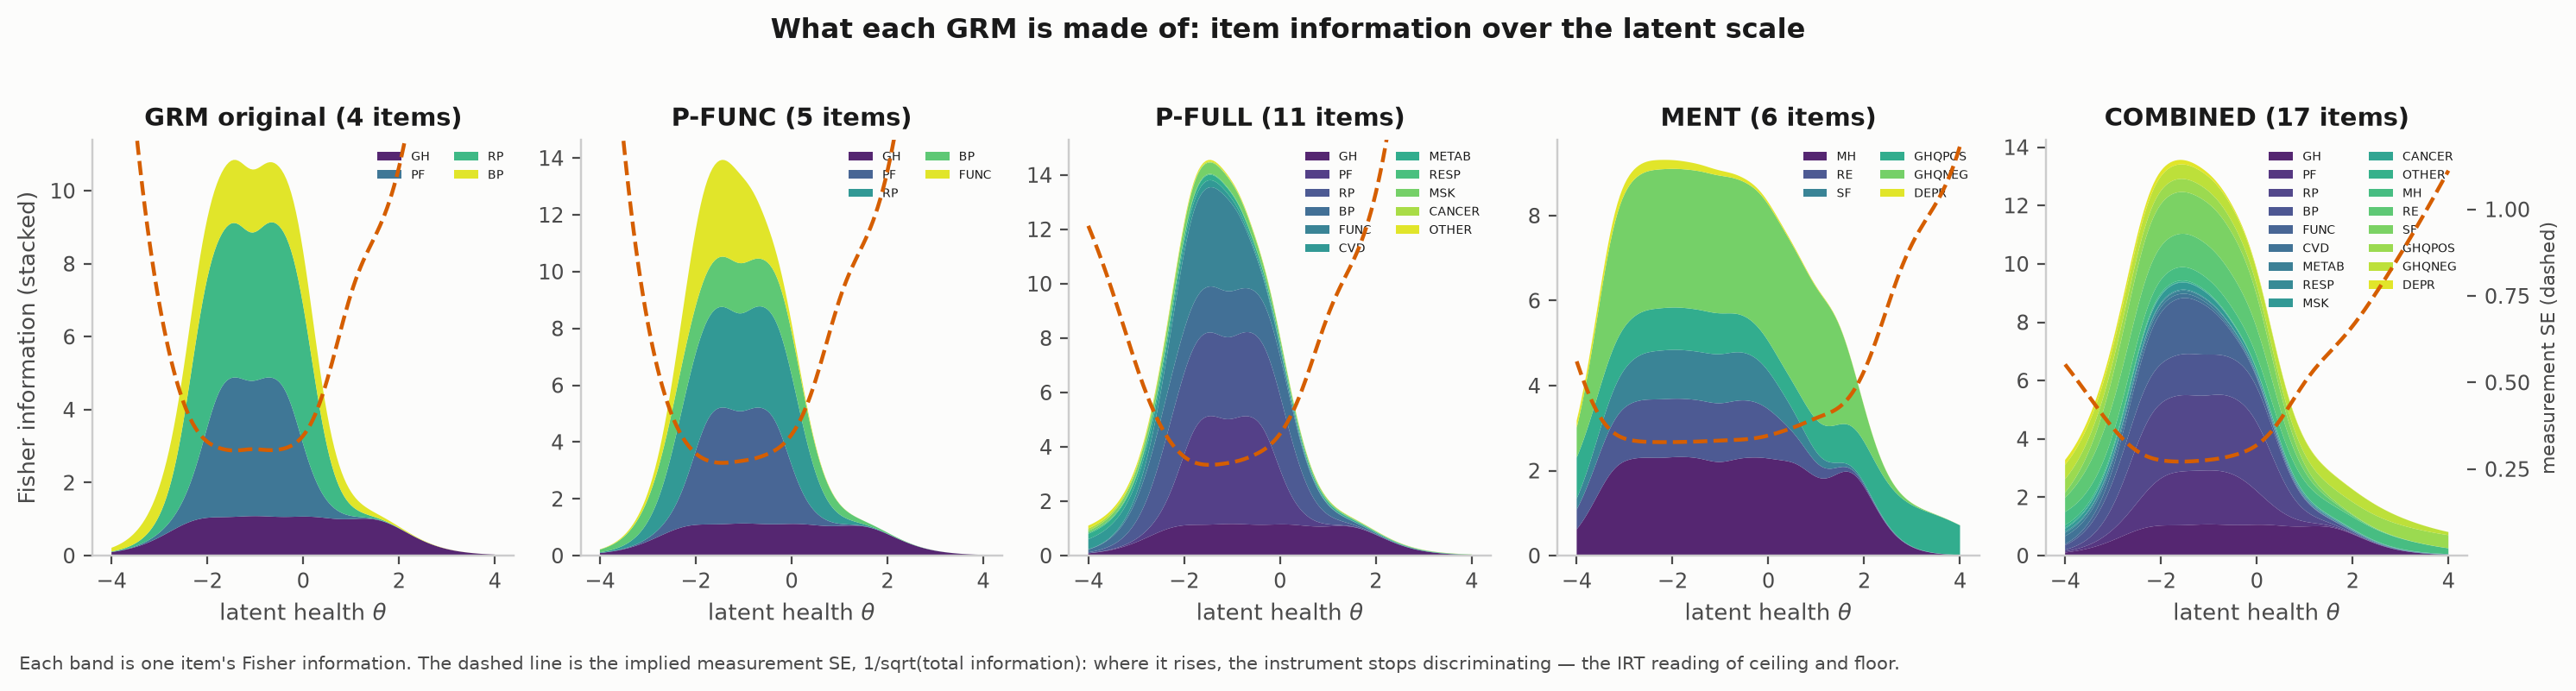
\includegraphics[width=\linewidth]{fig_grm_information}
\caption{What each GRM is made of: stacked item information over the latent
scale, with the implied measurement SE (dashed, right axis); each band is one
item, ordered as in the legend.
%
\emph{Panels:} \textbf{GRM original} is the four-testlet physical measure
replicated from the EIT note; \textbf{P-FUNC} adds the functioning testlet;
\textbf{P-FULL} adds the six diagnosis groups; \textbf{MENT} is the mental
bank; \textbf{COMBINED} is all seventeen items at once.
%
\emph{Physical items, from the SF-12:} \textbf{GH} general health (the single
self-rated-health question), \textbf{PF} physical functioning (moderate
activities, climbing stairs), \textbf{RP} role-physical (cutting down or
being limited at work because of physical health), \textbf{BP} bodily pain;
\textbf{FUNC} is the count of Equality Act physical limitations (mobility,
lifting, dexterity, coordination, personal care).
%
\emph{Diagnosis groups:} \textbf{CVD} cardiovascular events, \textbf{METAB}
diabetes and high blood pressure, \textbf{RESP} chronic airway disease,
\textbf{MSK} arthritis, \textbf{CANCER}, \textbf{OTHER} the pooled remainder
of thyroid, liver and epilepsy (\S\ref{sec:groups}).
%
\emph{Mental items:} \textbf{MH} mental health (calm; downhearted),
\textbf{RE} role-emotional (cutting down or working less carefully because of
emotional health), \textbf{SF} social functioning (health interfering with
social activities), \textbf{GHQPOS} and \textbf{GHQNEG} the positively- and
negatively-worded halves of the GHQ-12, \textbf{DEPR} ever-diagnosed clinical
depression.
%
FUNC adds a broad band of precision on the ill side; the condition items are
visibly thin; GHQ-negative dominates the mental bank; the combined bank is
tallest and widest but its SE still rises sharply above $\theta \approx +1$.}
\label{fig:info}
\end{figure}

\section{How the measures relate}

Correlations over all person-years (\code{descriptives/01}):

\begin{center}\small
\begin{tabular}{lccc}
\toprule
 & $\theta$ phys (FULL) & $\theta$ ment & $\theta$ combined \\
\midrule
original GRM (4 testlets) & \textbf{0.985} & 0.48 & 0.92 \\
UKHLS PCS & 0.904 & 0.23 & 0.76 \\
physical-only composite & 0.946 & 0.48 & 0.90 \\
UKHLS MCS & 0.27 & \textbf{0.882} & 0.58 \\
GHQ-12 Likert & $-0.38$ & $\mathbf{-0.904}$ & $-0.64$ \\
SF-6D utility & 0.71 & \textbf{0.799} & 0.88 \\
chronic count & $-0.58$ & $-0.21$ & $-0.51$ \\
$\theta$ phys $\times$ $\theta$ ment & \multicolumn{3}{c}{\textbf{0.457}} \\
\bottomrule
\end{tabular}
\end{center}

Three reads. The physical GRM is the object the project already validated,
with functioning attached. The mental GRM is the MCS/GHQ construct without
the orthogonality artifact. SF-6D correlates \emph{more} with the mental
theta (0.80) than the physical one (0.71) --- and its closest cousin is the
\emph{combined} bank (0.88): the SF-6D was a mixed measure all along.

\begin{figure}[H]
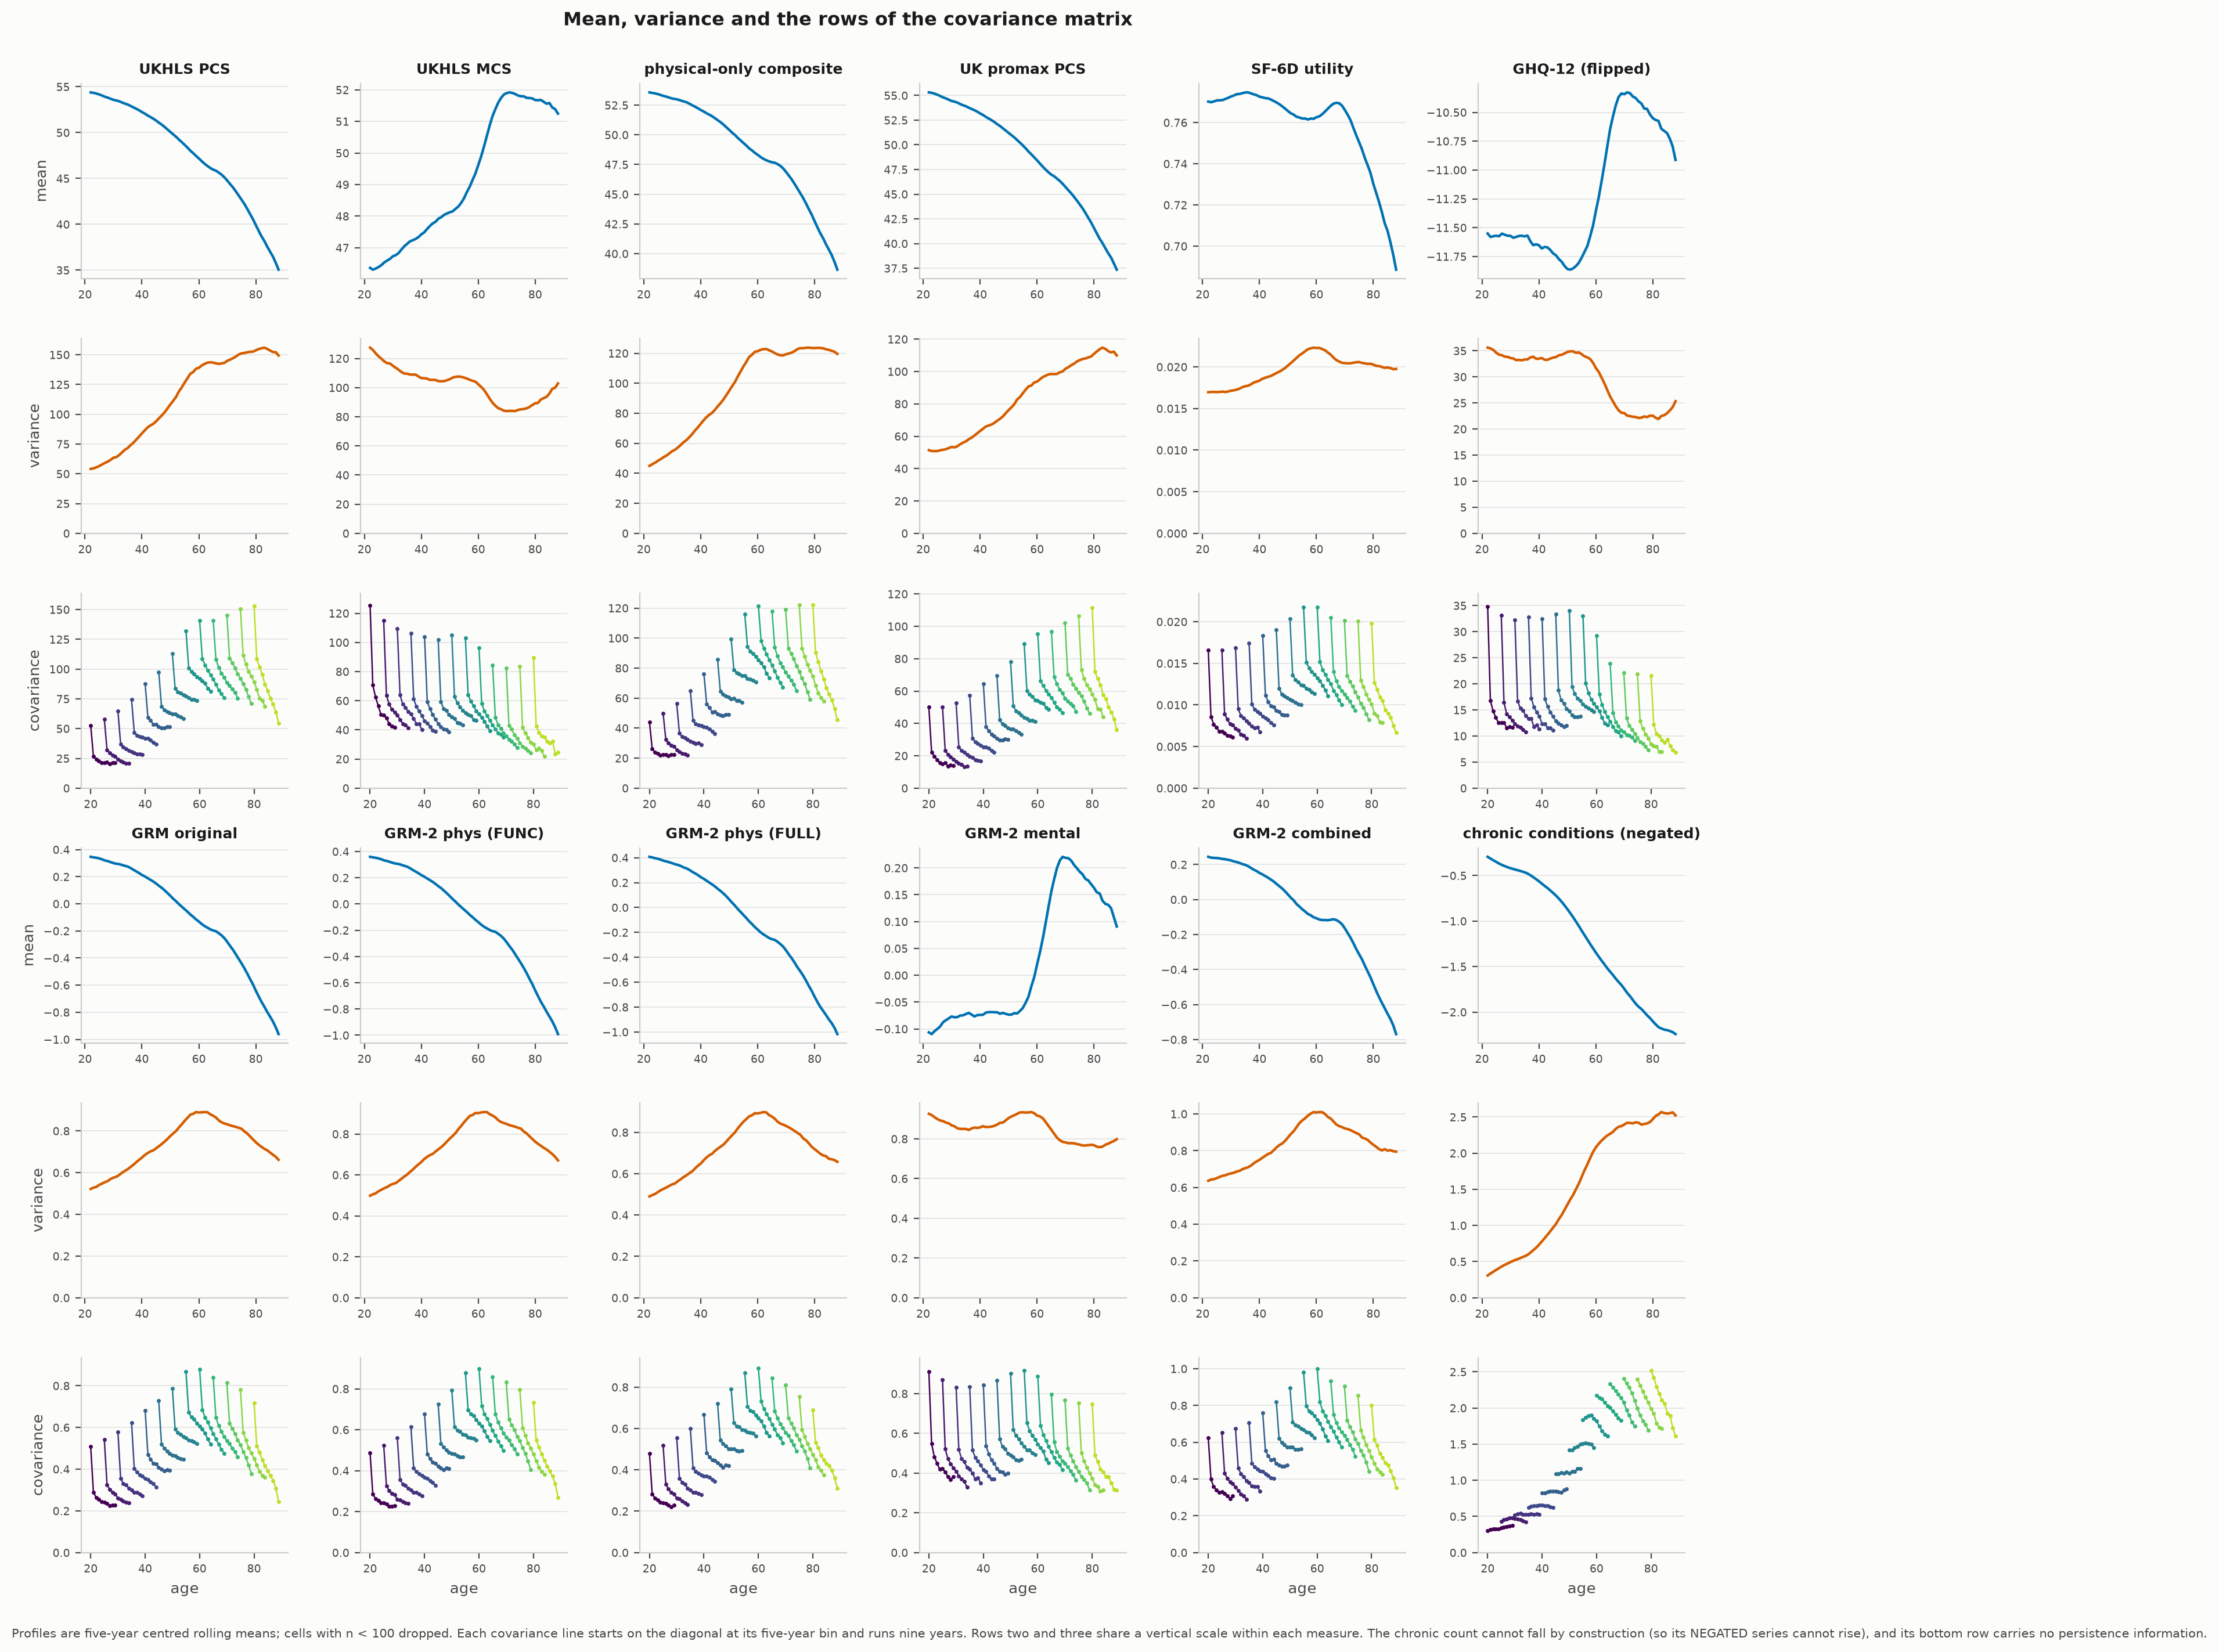
\includegraphics[width=\linewidth]{fig_moments_grid}
\caption{Mean, variance and the rows of the covariance matrix (the empirics
note's anatomy) for the full metric suite, two banks of six. GHQ and the
chronic count are \emph{negated}, so on every panel higher means better
health. The mental family (MCS, GHQ, mental GRM) shows the textbook late-life
wellbeing improvement; the physical measures share one anatomy ---
accelerating mean decline, rising-then-plateauing dispersion, fanning
covariance rows; the chronic count gives the physical mean and variance reads
from items fully disjoint from the SF-12, while its covariance row carries no
persistence information because the count cannot fall (so its negated series
cannot rise).}
\label{fig:moments}
\end{figure}

Two cautions on the mental hump, because on an auto-scaled axis it looks
dramatic. It is modest in size: mean GHQ falls from $11.75$ at age 55 to
$10.24$ at 70, which on a $0$--$36$ scale with a standard deviation of $5.62$
is $0.27$ sd; the axis spans less than two points, which is what makes it
read as a step change. And \emph{most of it is composition rather than
ageing}: among the 1{,}461 people observed in both windows, mean GHQ improves
by only $0.44$ points between ages 53--57 and 68--72, against a
cross-sectional gap of $1.42$ over the same ages, so under a third of the
apparent improvement survives holding the people fixed. The remainder is
selective non-response and attrition --- GHQ completion falls from $91\%$ at
age 70 to $77\%$ at 90 --- together with cohort differences. This applies to
every panel of the figure: these are pooled cross-sections in which age,
cohort and period are confounded, and they are descriptive scaffolding rather
than within-person trajectories. The mixture models of \S\ref{sec:ar1} do use
within-person information and are not subject to it.

\begin{figure}[H]
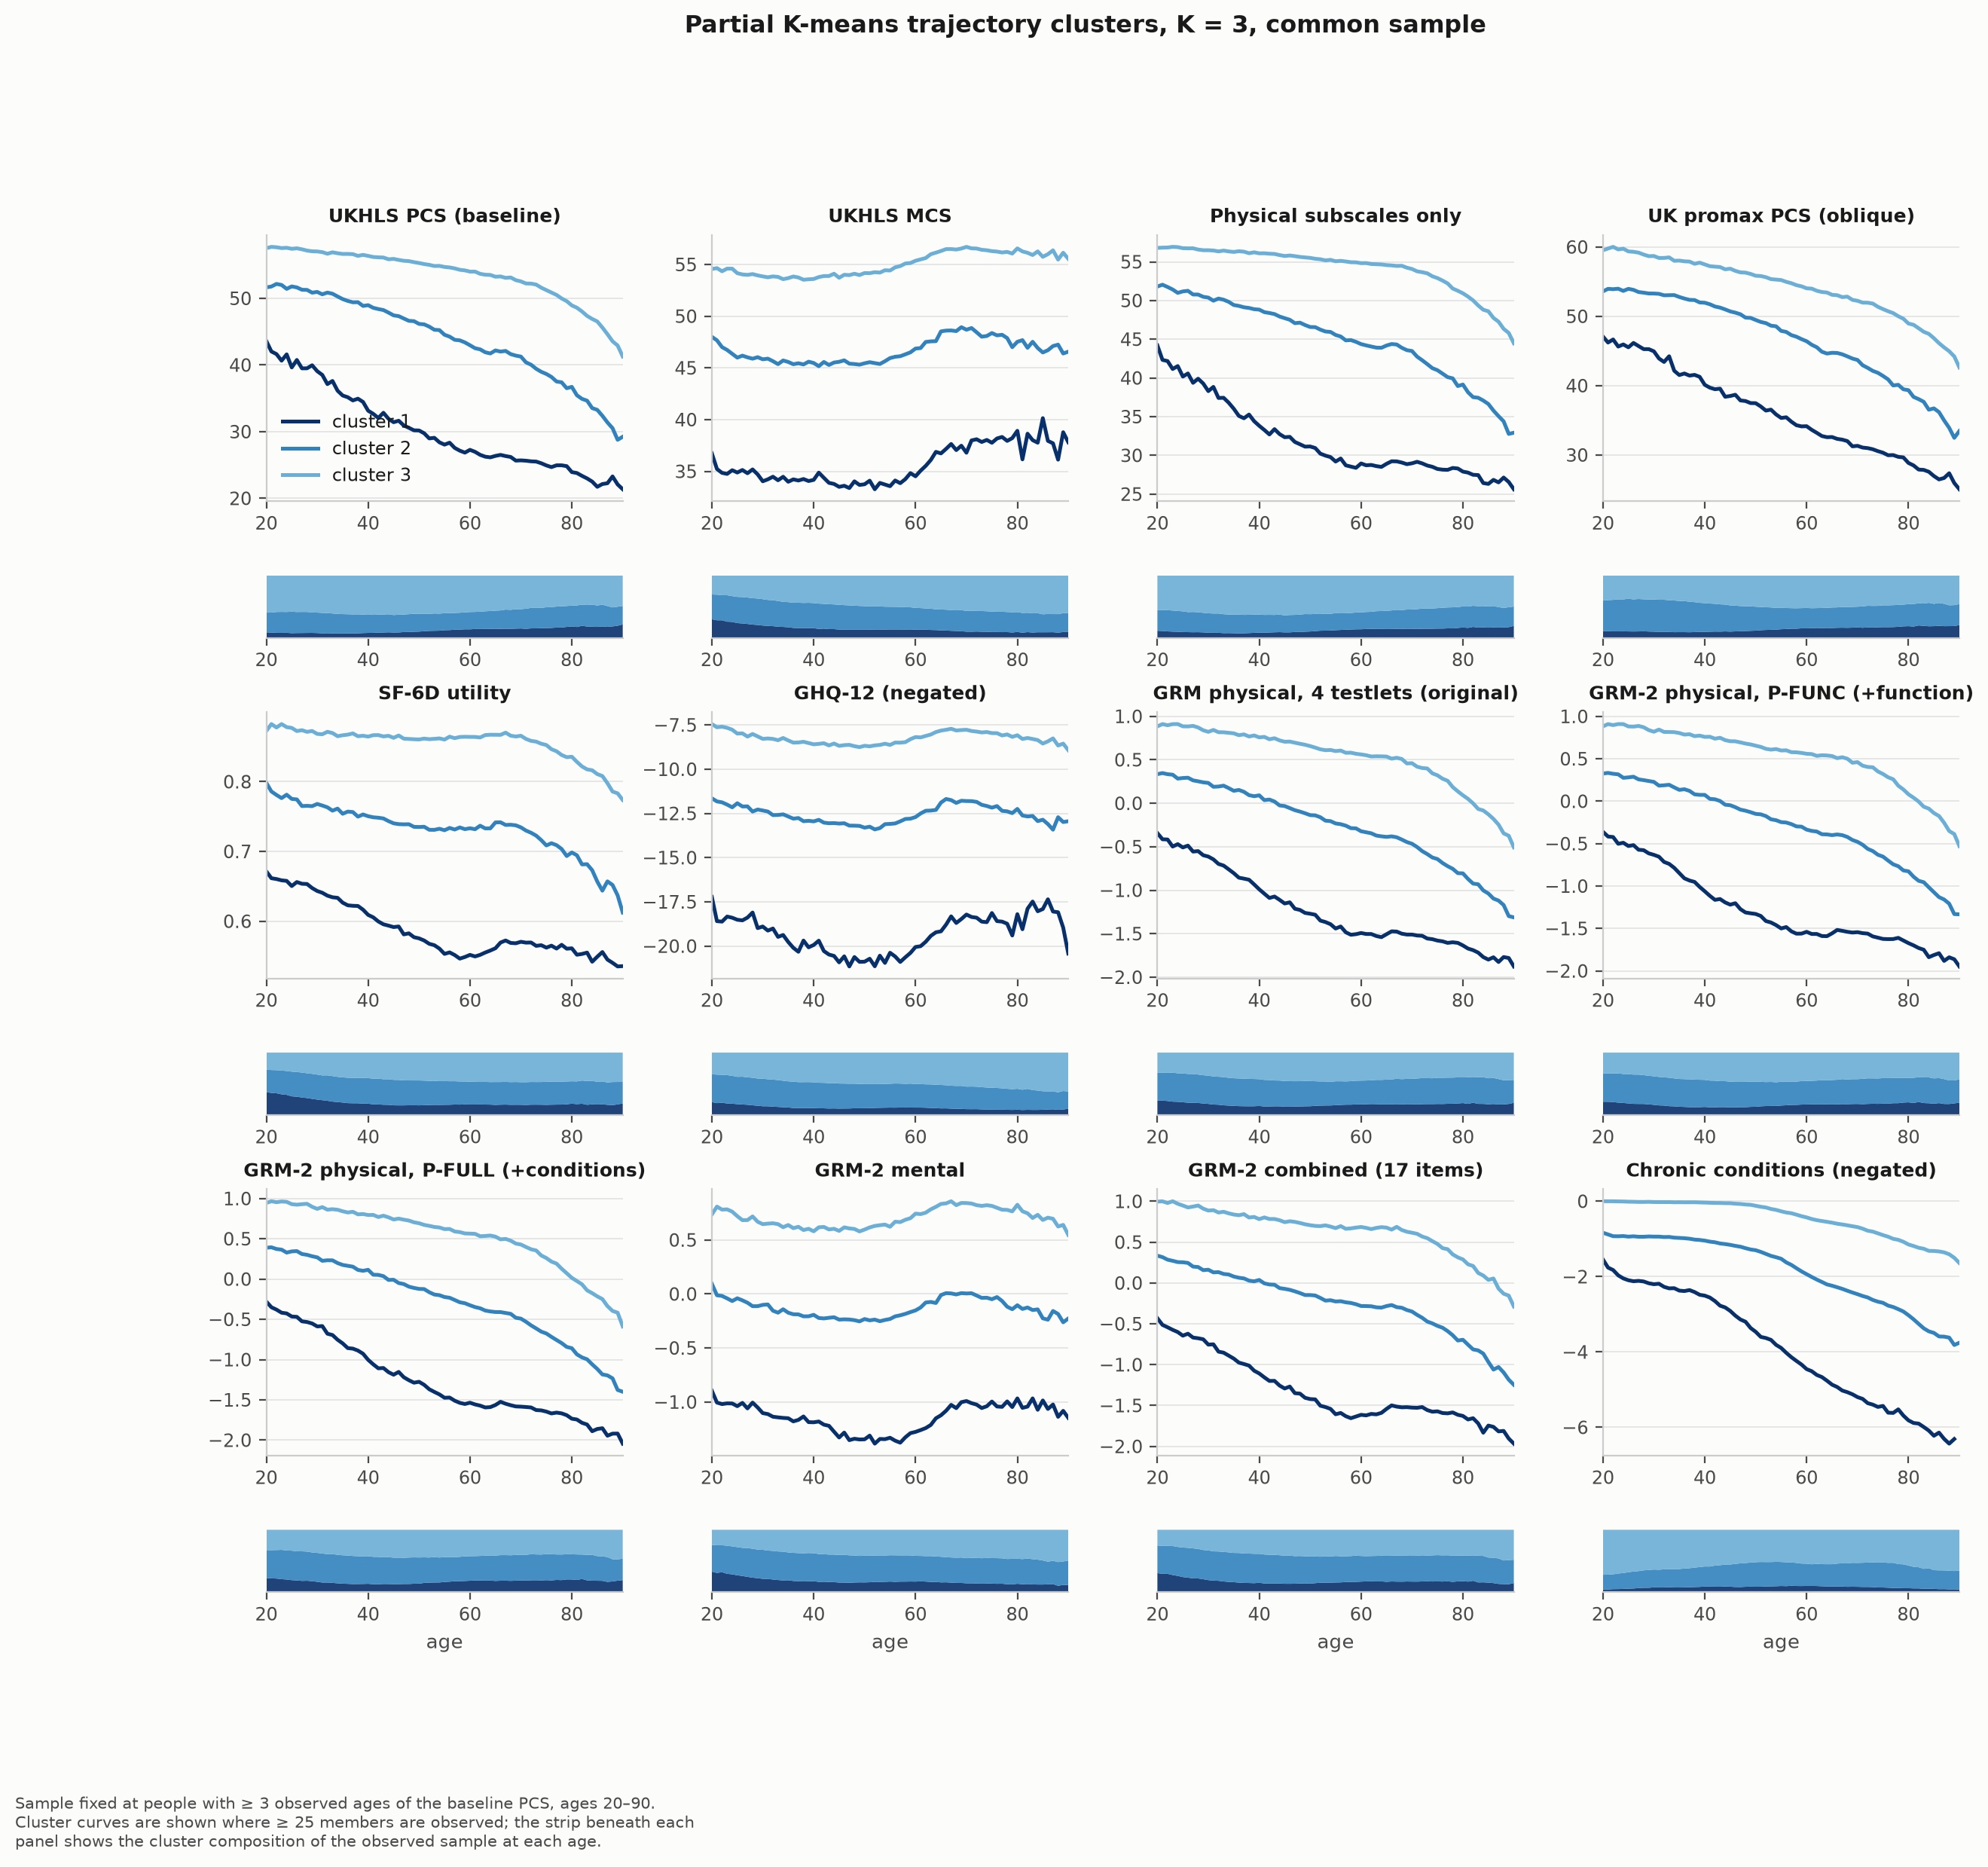
\includegraphics[width=\linewidth]{fig_cluster_trajectories}
\caption{Partial K-means trajectory clusters ($K=3$, 50 seeded inits,
sample fixed at people with $\ge 3$ observed baseline-PCS ages, ages
20--90), across the same twelve measures as Figure~\ref{fig:moments}. GHQ and
the chronic count are negated so every panel runs higher = better health. The
chronic count is monotone by construction, so its three bands can only fall
and never cross --- a property of the measure, not a finding about people.}
\label{fig:clusters}
\end{figure}

Partial K-means (Figure~\ref{fig:clusters}): changing the \emph{scoring}
moves the typology modestly while changing the \emph{construct} redraws it.
Against the PCS baseline, on the common sample:

\begin{center}\small
\begin{tabular}{lrrr}
\toprule
Measure & ARI & \% same cluster & chance \\
\midrule
Physical subscales only & \textbf{0.667} & 87.9 & 43.0 \\
UK promax PCS (oblique) & 0.464 & 79.4 & 39.5 \\
P-FUNC & 0.442 & 76.9 & 38.1 \\
GRM original (4 testlets) & 0.425 & 75.6 & 37.7 \\
P-FULL & 0.409 & 74.9 & 37.5 \\
GRM combined (17 items) & 0.266 & 66.1 & 36.8 \\
SF-6D utility & 0.185 & 60.0 & 37.4 \\
Chronic conditions (negated) & 0.120 & 56.1 & 44.3 \\
GHQ-12 (negated) & 0.079 & 51.4 & 40.8 \\
GRM mental & 0.074 & 49.2 & 37.1 \\
UKHLS MCS & \textbf{0.053} & 48.0 & 40.0 \\
\bottomrule
\end{tabular}
\end{center}

The physical measures agree substantially with the baseline whatever the
scoring --- 0.41 to 0.67 --- and the ordering is instructive: the composite
that merely re-weights the same subscales agrees most, the IRT re-spacings
sit in the middle, and the further a measure moves from the PCS's item set
the lower it falls. The mental measures sit at the bottom, essentially at
chance: MCS at ARI 0.053 and the mental GRM at 0.074, with same-cluster rates
of 48\% and 49\% against chance rates of 40\% and 37\%. The combined bank
lands between the two families at 0.27, which is what a physically-dominated
mixture of them should do. So the physical typology is robust to how physical
health is scored, and the mental dimension partitions people almost
independently of it --- the same conclusion the two-bank correlation of
$0.457$ reaches by a different route.

\section{The ever-diagnosis question, resolved}
\label{sec:ever}

The misgiving: historical diagnoses accumulate mechanically with age, so a
diagnosis-bearing measure could manufacture ``decline'' out of stale
paperwork. Four reads.

\begin{figure}[H]
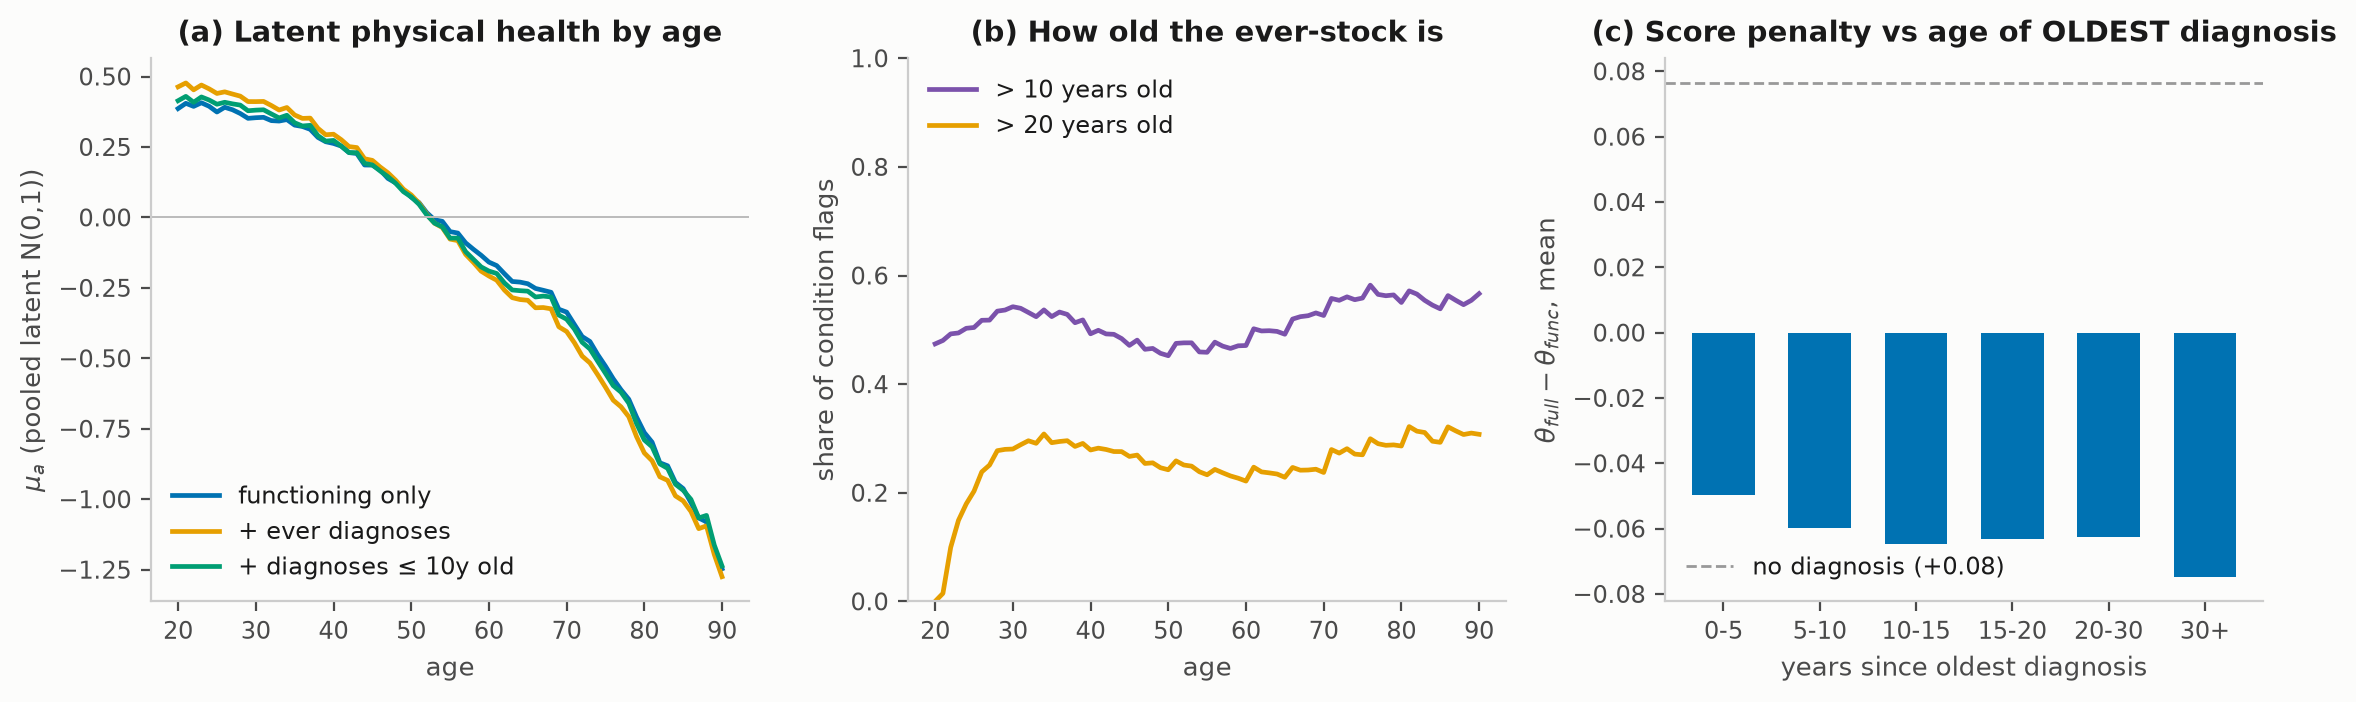
\includegraphics[width=\linewidth]{fig_ever_sensitivity}
\caption{The ever-diagnosis question, all three panels on the physical
GRM. (a) latent age profiles $\mu_a$ under P-FUNC (functioning only), P-FULL
(plus ever-diagnoses) and P-REC (plus diagnoses at most ten years old); (b)
the staleness of the UKHLS chronic-condition stock; (c) the per-person gap
$\theta_{\text{P-FULL}} - \theta_{\text{P-FUNC}}$ against the age of that
person's oldest diagnosis.}
\label{fig:ever}
\end{figure}

\textbf{(1) The aggregate effect is real but bounded.}
$\mu(80)-\mu(30)$ is $-1.117$ SD functioning-only, $-1.247$ with
ever-diagnoses, $-1.170$ with only diagnoses $\le$10 years old. Diagnoses
steepen the measured lifecycle decline by 0.130 SD (12\%), and 59\% of that
extra steepness comes from diagnoses more than a decade old --- leaving the
stale-accumulation component at $\sim$6\% of the total decline.

\textbf{(2) The potential was much larger than the realised effect.} Half
the ever-stock is $>$10 years old at every age past 40 (\S2.4). The damage
stays small because the estimator protects itself: items that cannot predict
the functioning responses get low discriminations, so stale-heavy condition
items simply carry little weight.

\textbf{(3) The items cannot tell stale from fresh --- which cuts both
ways.} The person-level penalty $\theta_{\mathrm{full}} -
\theta_{\mathrm{func}}$ is flat in the age of the oldest diagnosis ($-0.05$
SD at 0--5 years, $-0.075$ at 30+). Read as measurement of \emph{current}
health, that is exactly the mechanism feared: no within-item discounting
exists. It is an argument \emph{against trusting ever-items as current-state
measures}, and simultaneously the reason their damage is capped.

\textbf{(4) Asked directly, the data mostly decline to discount.} P-TIMED
splits every group into recent ($\le$10y) and stale ($>$10y) items and lets
the model estimate their separate discriminations --- the in-framework
analogue of an estimated recency-weight function:

\begin{center}\small
\begin{tabular}{lccc}
\toprule
Group & $a$ recent & $a$ stale & ratio \\
\midrule
CVD & 1.19 & 1.21 & 0.99 \\
METAB & 0.59 & 0.81 & 0.72 \\
RESP & 0.68 & 0.29 & \textbf{2.31} \\
MSK & 0.83 & 1.22 & 0.68 \\
CANCER & 0.59 & 0.56 & 1.05 \\
OTHER & 0.63 & 0.63 & 1.00 \\
\bottomrule
\end{tabular}
\end{center}

Only respiratory disease wants a discount (remitting childhood asthma). For
arthritis and the metabolic conditions the \emph{stale} item is more
informative --- progressive diseases, where an old diagnosis means longer
duration and worse current health. The mechanistic-accumulation story is
really a story about \emph{remitting} conditions; for progressive conditions
the old diagnosis is legitimately informative.

\textbf{Related literature.} Estimating recency weights on past exposures is
the weighted-cumulative-exposure literature (Sylvestre \& Abrahamowicz 2009;
review in Kelly et al.\ 2024; R package \code{WCE}), with spline-estimated
weight-by-recency functions --- P-TIMED is its two-knot IRT analogue.
Letting item parameters vary continuously with a covariate such as time
since diagnosis is moderated nonlinear factor analysis (Bauer \& Hussong
2009; regularised variants for DIF detection), the natural next refinement
if a smooth weighting is ever needed. The simpler administrative-data
practice is a fixed lookback window (Preen et al.\ 2006), which P-REC
implements. Health-state valuation handles the same issue with acute
vs.\ post-acute utilities for events like stroke.

\textbf{Verdict.} For lifecycle \emph{dynamics}, use P-FUNC (or the original
GRM, $r=0.994$): a pure current-state instrument. P-FULL is a sound
descriptive companion whose accumulation bias is now characterised and
bounded ($\sim$0.08--0.13 SD over the lifecycle, concentrated in remitting
conditions); P-REC and P-TIMED are its sensitivity band. Where conditions
matter substantively, model them as separate channels in the Bayesian
mixture, where ``ever'' is the correct state variable.

\section{One dimension or two? The combined GRM}
\label{sec:combined}

The combined bank (all seventeen items, one latent dimension) fits, scores,
and correlates sensibly ($r=0.92$ with the physical bank, 0.75 with the
mental, 0.88 with SF-6D). But it fails the assumption the others satisfy:
after conditioning on its single dimension, the mental items remain strongly
positively correlated --- $Q_3(\mathrm{MH}, \mathrm{GHQ}^-)=+0.58$,
$Q_3(\mathrm{GHQ}^+, \mathrm{GHQ}^-)=+0.54$, $Q_3(\mathrm{MH},
\mathrm{RE})=+0.33$ --- while the physical side stays clean (max
phys--phys $Q_3$ $+0.20$). That residual clustering is the data saying the
mental items share a dimension the combined score cannot represent: with
$r(\theta_P,\theta_M)=0.457$, one dimension is a genuine misspecification,
not a summary. The same criteria table shows the cost in substance: the
combined score reintroduces a mental-health artifact of $-0.82$ SD at a
fixed physical profile (the physical banks: $0.00$), and its cohort spread
collapses to 0.06 SD not because it is clean but because physical health
improving and mental health deteriorating across cohorts \emph{cancel}
inside it --- precisely the mixing the EIT note warned about. Use it only
where a single index is externally imposed; a bifactor model (general +
physical/mental group factors) would be the defensible one-number
construction if that need becomes real.

\begin{figure}[H]
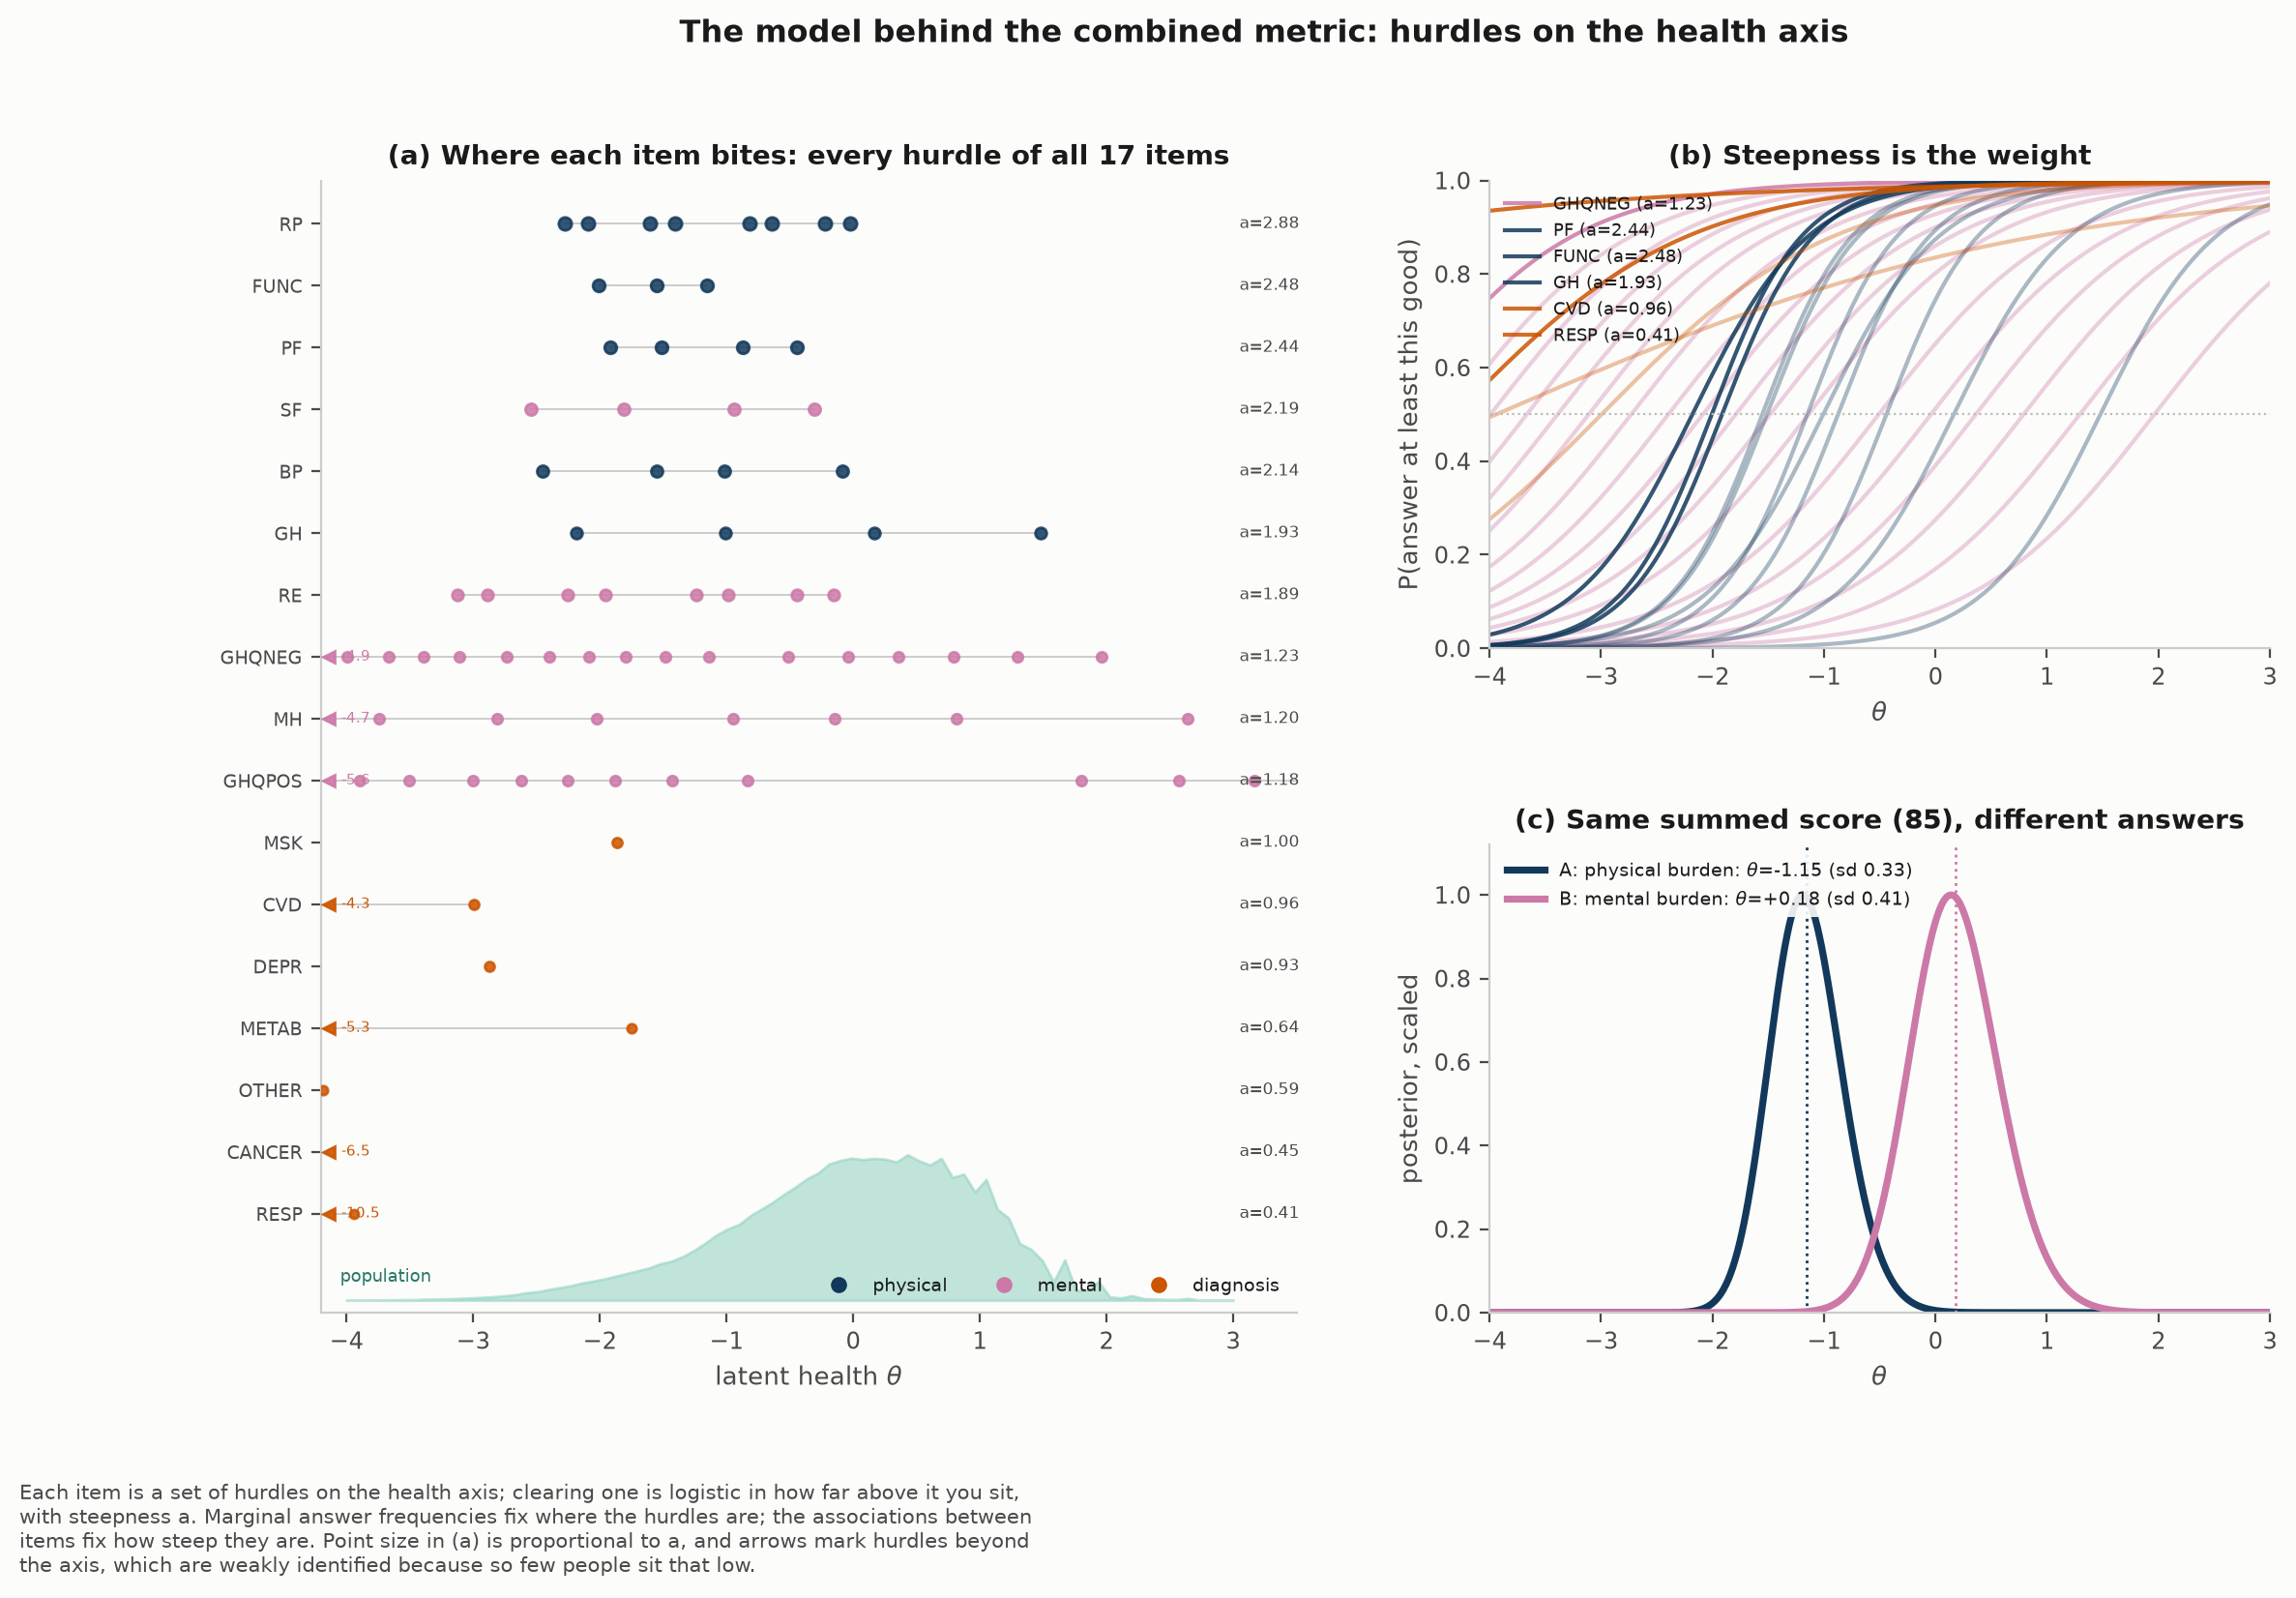
\includegraphics[width=\linewidth]{fig_combined_grm_model}
\caption{The model behind the combined metric, in the empirics note's
hurdles-on-the-health-axis form, for the most all-encompassing bank. (a)
every hurdle of all seventeen items against the population distribution of
$\theta$; (b) the hurdle curves for items spanning the weight range; (c) two
people whose category numbers sum to the same total.}
\label{fig:combmodel}
\end{figure}

Figure~\ref{fig:combmodel} draws the combined bank as a set of hurdles.
Panel (a) makes the division of labour visible: the physical items (RP, FUNC,
PF, BP, GH; $a = 1.9$--$2.9$) cluster their hurdles between $-2.5$ and $0$,
the mental items (GHQNEG, MH, GHQPOS; $a = 1.2$) spread theirs across the
whole axis and beyond it, and the diagnosis items ($a = 0.4$--$1.0$) sit far
to the left. Panel (c) then shows what that means for a score. Two people
whose answers sum to exactly the same total --- one carrying the deficit on
the physical items, the other on the mental ones --- receive
$\theta = -1.15$ and $\theta = +0.18$, a gap of $1.3$ standard deviations.
The combined bank is not a balanced physical--mental index; it is
physically dominated, because the physical items are the steeper and hence
the more reliable ones. That is a second, independent reason (alongside the
residual clustering of \S\ref{sec:combined}) to prefer the two-bank design.

\begin{figure}[H]
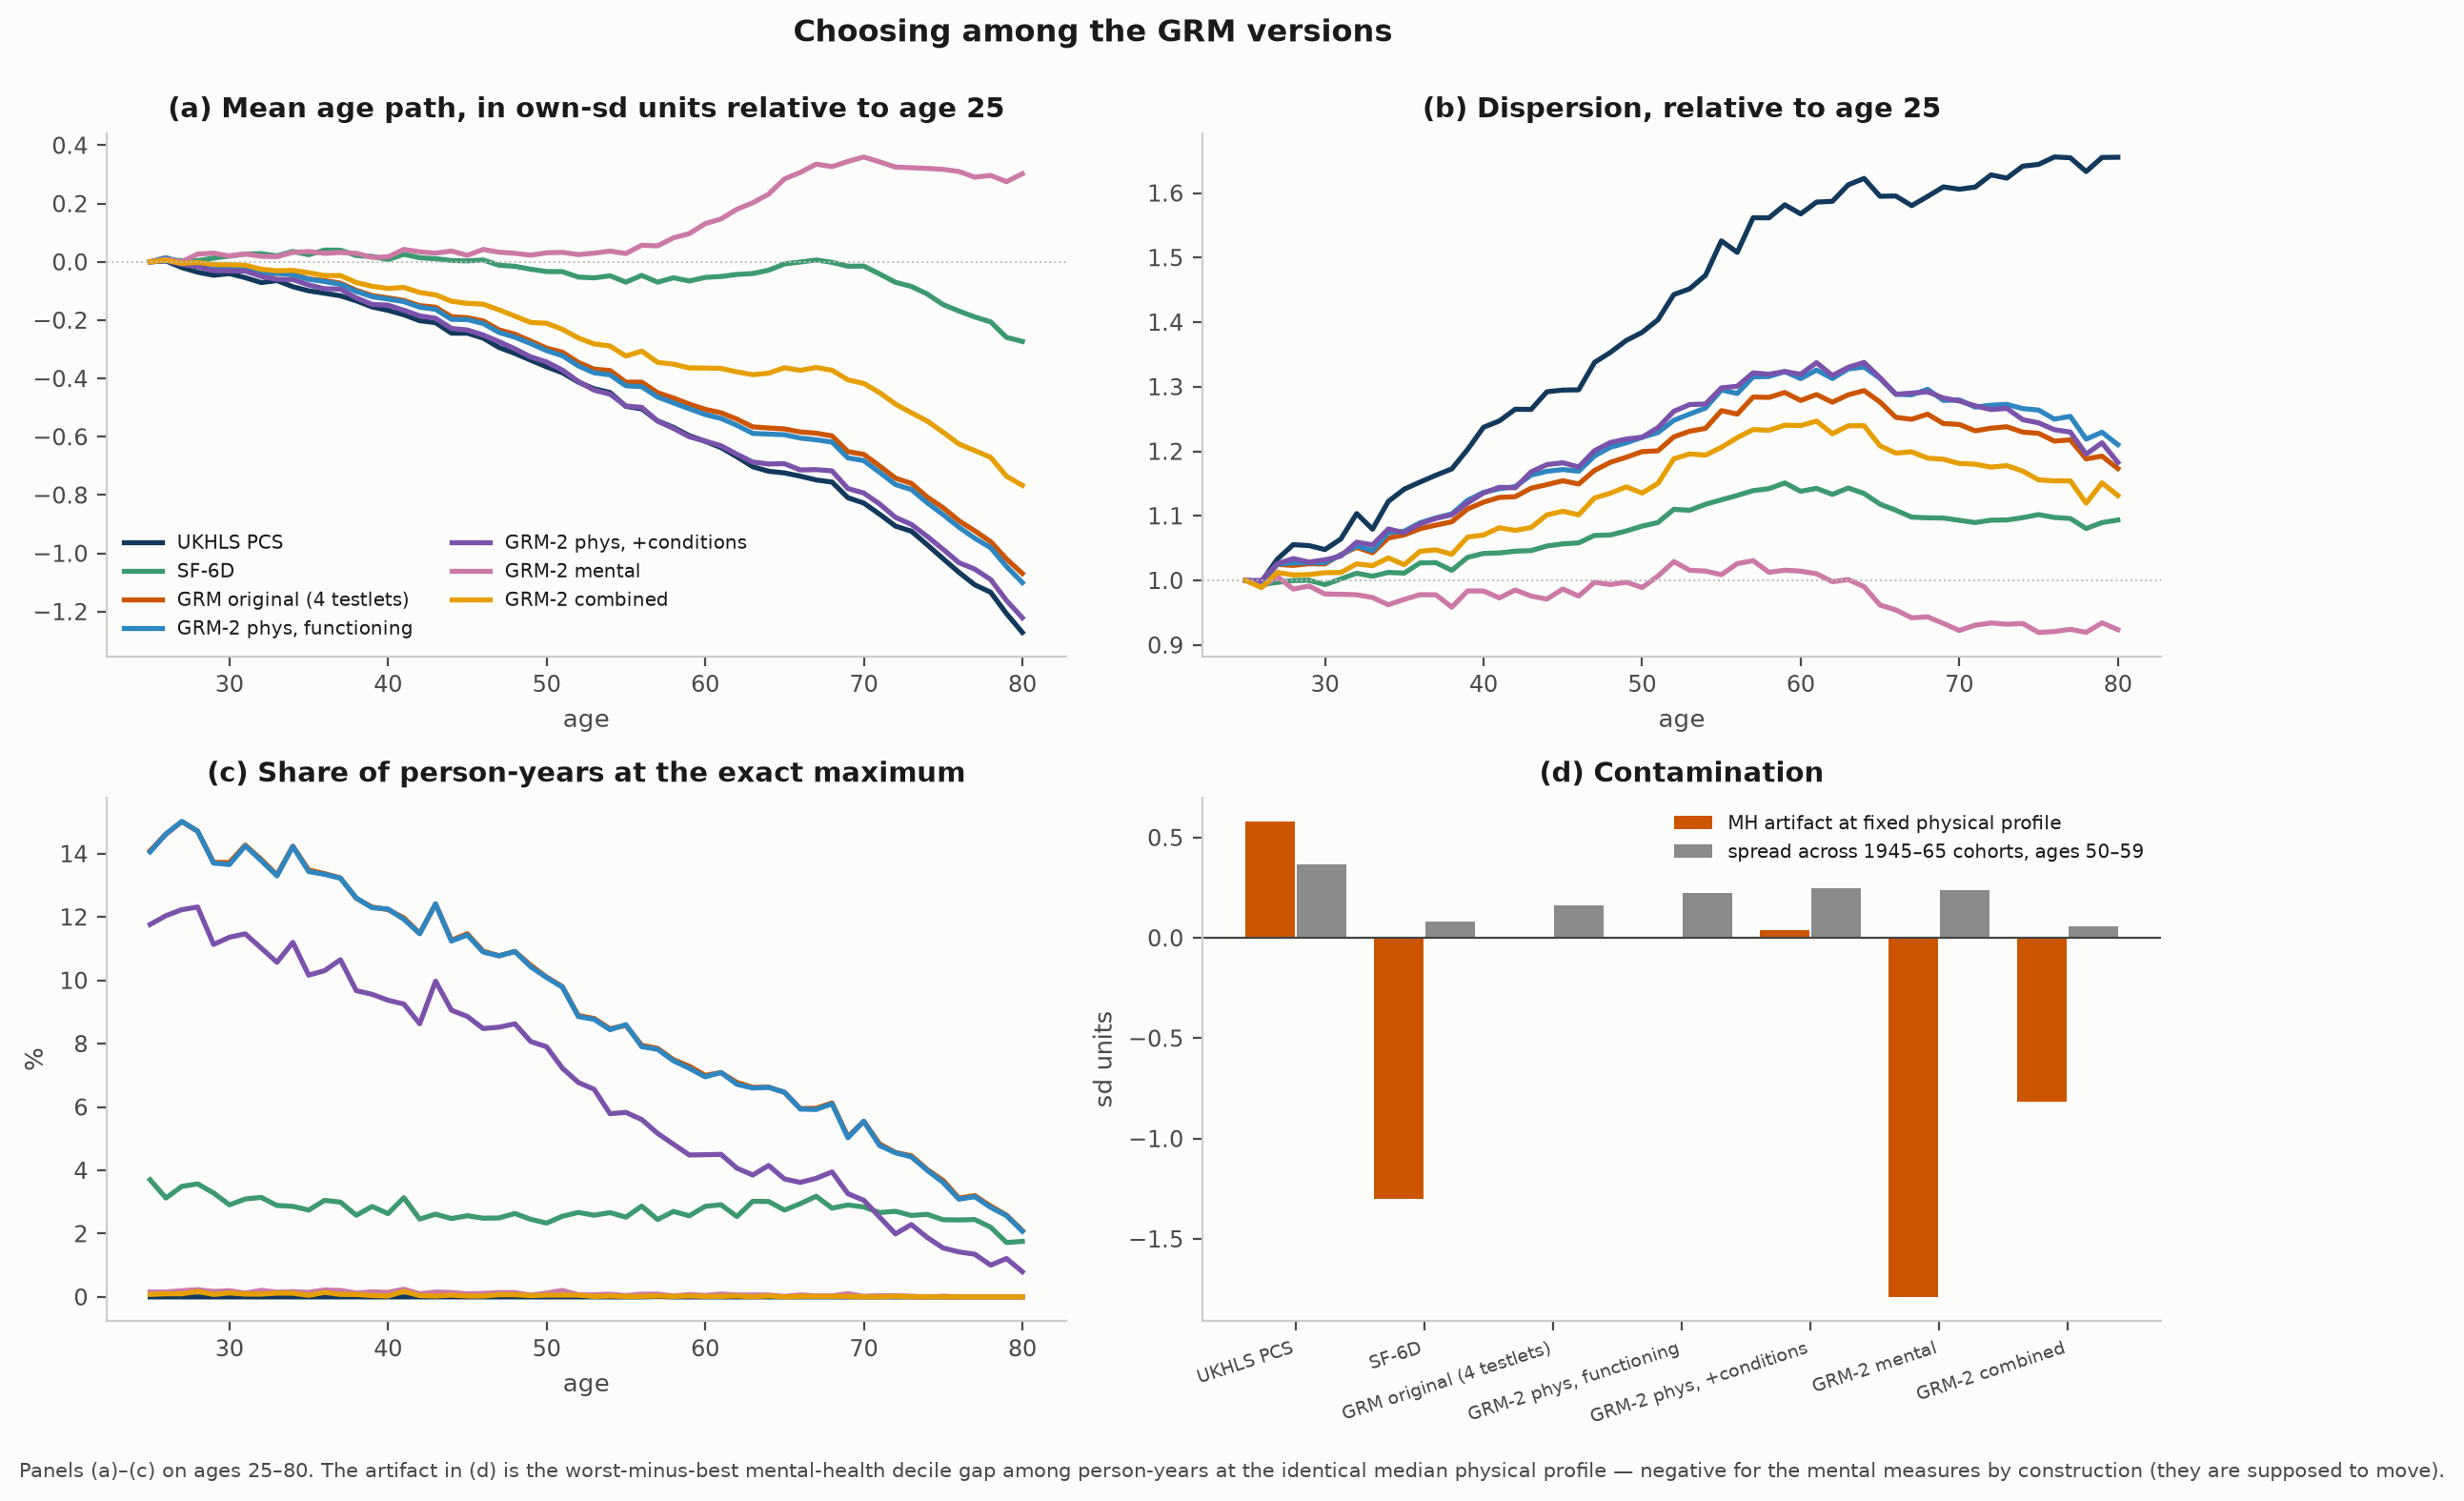
\includegraphics[width=\linewidth]{fig_grm_versions}
\caption{The measure-choice panel across measures (the empirics note's
Figure 30, rebuilt): mean age path, dispersion, how much room each measure
has left at its two limits, and the two contamination reads. Seven measures:
UKHLS PCS, SF-6D utility, the original four-testlet GRM, P-FUNC, P-FULL, the
mental GRM and the combined GRM. Panel (c) now carries both limits --- the
solid line is the share of person-years at the measure's exact maximum, the
dashed line, mirrored below zero, the share at its exact minimum, and both
are read as positive percentages. The asymmetry is the point: ceiling mass
runs to $15\%$ at the young end while floor mass never exceeds about $1.5\%$
anywhere, so these instruments run out of room among the healthy long before
they do among the ill.}
\label{fig:versions}
\end{figure}

\section{Ceiling and floor}
\label{sec:ceiling}

Two different questions hide under ``ceiling effects'': how much probability
mass sits at the best attainable response profile, and whether the
instrument can \emph{discriminate} among the healthy. More items help
enormously with the first and only marginally with the second.

\begin{center}\small
\begin{tabular}{lrrrrr}
\toprule
Measure & ceiling \% & floor \% & range (sd units) & psd at top & psd at bottom \\
\midrule
UKHLS PCS (12 items) & 0.89$^{a}$ & $\sim$0 & 6.5 & --- & --- \\
Physical-only composite & 9.95 & 0.91 & 4.1 & --- & --- \\
SF-6D utility & 2.98 & 0.18 & 4.7 & --- & --- \\
GHQ-12 Likert & 0.20 & 0.31 & 6.4 & --- & --- \\
GRM original (4 testlets) & 9.55 & 0.97 & 4.4 & 0.65 & 0.45 \\
P-FUNC & 9.53 & 0.76 & 4.5 & 0.65 & 0.44 \\
P-FULL & 7.16 & 0.00 & 5.3 & 0.64 & 0.56 \\
MENT & 0.11 & 0.03 & 6.5 & 0.60 & 0.45 \\
COMBINED & 0.05 & 0.00 & 7.5 & 0.66 & 0.55 \\
\bottomrule
\end{tabular}

{\scriptsize $^{a}$share at the all-best 12-item profile (the exact-maximum
read is degenerate for a continuous derived score). ``psd'' is the EAP
posterior sd at the all-best / all-worst response pattern.}
\end{center}

The optimistic half of the hypothesis is confirmed: ceiling mass collapses
from 9.5\% (original GRM) to 7.2\% with conditions and to 0.05--0.11\% for
the mental and combined banks, and the floors of P-FULL and COMBINED empty
entirely. Panel (c) of Figure~\ref{fig:versions} shows where it binds: the
young end, where the physical banks still park 12--15\% of person-years at
the maximum.

The pessimistic half is also right, and Figure~\ref{fig:info} shows why: the
posterior sd at the very top is $\sim$0.6--0.66 \emph{for every version} ---
seventeen items buy no more precision among the healthy than four, because
every added item has strongly negative thresholds (all these instruments
measure ill-health). Extra items \emph{spread} the top mass into a finer
ranking (ties broken by GHQ and diagnoses) without adding information where
the healthy live. Genuinely fixing the ceiling requires items with positive
thresholds --- vigorous-functioning items of the PROMIS physical-function
type --- which UKHLS does not carry. For the mixture models this is a
manageable, known feature: the likelihood sees ordered categories, not the
score, and the ceiling category is one of them.

\subsection*{The floor, in depth}

The floor is the mirror image, and here the added items genuinely work ---
their negative thresholds sit exactly where the severely ill live
(\code{descriptives/06}, \code{floor\_depth.csv}):

\begin{center}\small
\begin{tabular}{lccccccc}
\toprule
 & \multicolumn{3}{c}{measurement SE at $\theta=$} & min & \% $<-3$ &
\% at worst & distinct $\theta$ in \\
 & $-4$ & $-3$ & $-2$ & $\theta$ & & pattern & bottom 1\% \\
\midrule
GRM original & 2.15 & 0.73 & 0.33 & $-2.61$ & 0.00 & 0.97 & \textbf{2} \\
P-FUNC & 2.12 & 0.67 & 0.30 & $-2.68$ & 0.00 & 0.76 & 3 \\
P-FULL & \textbf{0.95} & \textbf{0.55} & 0.29 & $-3.38$ & 0.03 & 0.00 & \textbf{575} \\
MENT & 0.56 & 0.34 & 0.33 & $-3.72$ & 0.30 & 0.03 & 1{,}524 \\
COMBINED & \textbf{0.55} & \textbf{0.37} & 0.28 & $-4.43$ & 0.24 & 0.00 & 3{,}708 \\
\bottomrule
\end{tabular}
\end{center}

A note on reading Figure~\ref{fig:info}: P-FULL carries visible information
out to the left edge of the axis where the other physical banks have none.
That is real measurement, not an artefact of where the axis stops. Total test
information at $\theta = -4$ is $1.10$ for P-FULL against $0.22$ for P-FUNC,
and at $\theta = -6$ it is $0.37$ against $0.00$; the axis is not hiding a
cliff, the curve simply keeps declining. The information there comes almost
entirely from the diagnosis items --- CVD ($34\%$ of it), METAB ($18\%$),
OTHER ($10\%$) --- whose hurdles sit at $-3.6$ and $-4.1$, precisely in that
region. It is the opposite of a floor effect: a floor effect is information
\emph{collapsing} at the bottom, which is what the functioning-only banks do.
The caveat is that a few of these thresholds are weakly identified because so
few people sit that low (RESP's first hurdle is estimated at $-10.5$, CANCER's
at $-6.5$ in the combined bank), so the far tail should not be read as
precisely located --- but at $\theta = -4$ the contributing hurdles are all
within the range the data actually cover.

The original GRM (and P-FUNC) have a real floor problem: the instrument goes
dark below $\theta\approx-2.5$ (SE 0.7 at $-3$, 2.1 at $-4$), the scale
simply ends at $-2.6$, and the entire bottom percentile collapses onto two
or three response patterns --- the worst-off are a spike, not a
distribution. The condition items repair precisely this: their thresholds
($-2.6$ to $-4.6$) are the only ones deep in the ill tail, so P-FULL keeps
SE at 0.55 at $\theta=-3$, extends the scale to $-3.4$, empties the
worst-pattern spike entirely, and resolves the bottom percentile into 575
distinct positions. Among the P-FUNC bottom \emph{decile} (37.6k
person-years --- the population a prevention analysis targets), P-FUNC
distinguishes 1{,}252 values, P-FULL 16{,}522, COMBINED essentially one per
person-year. The mental bank has the best floor of all (GHQ thresholds reach
$-3.5$; SE 0.34 at $-3$).

This sharpens the ever-diagnosis trade-off of \S\ref{sec:ever}: the
diagnosis items' cost is a bounded accumulation bias in the age gradient;
their benefit is measurement depth among the severely ill, which
functioning items alone cannot provide because severe limitation saturates
them. For analyses that turn on the worst-health group --- describing the
bottom class, targeting --- P-FULL is the better physical instrument; for
population dynamics, P-FUNC remains the clean choice.

\section{Convexity against healthcare use}
\label{sec:convexity}

Is healthcare use convex in health --- falling steeply among the ill, flat
among the healthy --- and does each metric's cardinalisation carry that
shape? Following the construction-note convexity exercise, each outcome is
regressed on the standardised measure and its square on a common sample
(waves 7--15, all fifteen
measures observed; $n = 209{,}042$ in-patient, $208{,}936$ out-patient), with
measures oriented so higher = better: on a declining relationship, a
positive quadratic = convex. One data correction first: UKHLS mainstage has
\emph{no GP-visit count}. \code{hl2gp}, despite its name, is labelled
``hosp or clinic \emph{out-patient} last 12 months'' (the sandbox's ``GP
band'' was a mislabel, corrected here); the only GP variable is
\code{servuse1} (``service use: your local doctor'', yes/no, five waves),
included as a supplementary outcome.

\begin{figure}[H]
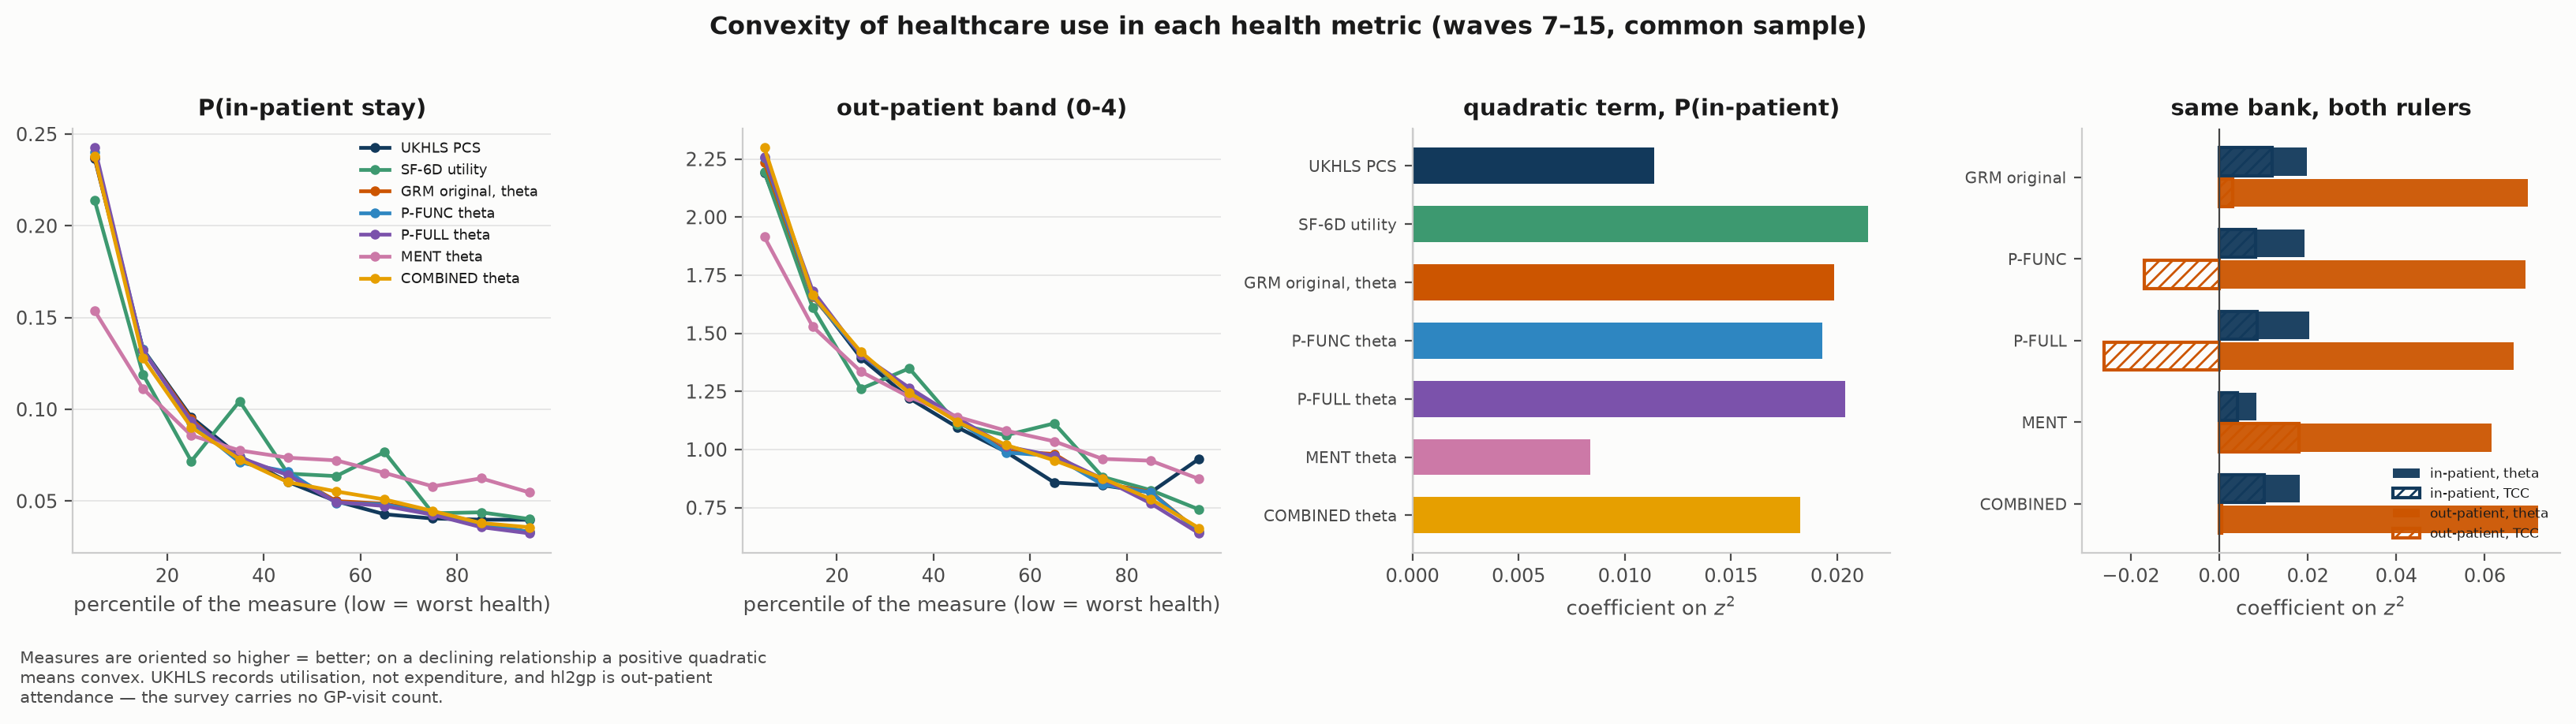
\includegraphics[width=\linewidth]{fig_convexity}
\caption{Healthcare use across the distribution of each measure, and the
quadratic (convexity) term for in-patient admission. All fifteen measures
are tested (Table above); the seven plotted in the first two panels are
UKHLS PCS, SF-6D utility, the original GRM, P-FUNC, P-FULL, the mental GRM
and the combined GRM, each oriented so higher means better health. The
fourth panel sets each bank's $\theta$ (solid) against its TCC (hatched) for
both outcomes: identical people, identical ranking, different units.}
\label{fig:convexity}
\end{figure}

\begin{center}\small
\begin{tabular}{lcccc}
\toprule
 & \multicolumn{2}{c}{quadratic term ($t$)} &
\multicolumn{2}{c}{$P(\text{in-patient})$} \\
Measure & in-patient & out-patient & bottom 1\% & top 1\% \\
\midrule
UKHLS PCS & $+.011$ (24) & $+.032$ (18) & .312 & .042 \\
UKHLS MCS & $+.004$ (8) & $+.038$ (22) & .128 & .134 \\
Physical-only composite & $+.011$ (22) & $+.002$ (1) & .331 & .033 \\
SF-6D utility & $+.021$ (40) & $+.119$ (61) & .289 & .039 \\
GHQ-12 (flipped) & $+.003$ (8) & $+.007$ (5) & .189 & .059 \\
\midrule
\multicolumn{5}{@{}l}{\emph{each bank on both rulers}} \\
GRM original, $\theta$ & $+.020$ (43) & $+.070$ (42) & .331 & .033 \\
GRM original, TCC & $+.012$ (23) & $+.003$ (2) & .331 & .033 \\
\addlinespace
P-FUNC $\theta$ & $+.019$ (42) & $+.069$ (42) & .322 & .033 \\
P-FUNC, TCC & $+.008$ (17) & $\mathbf{-.017}$ $(-9)$ & .322 & .033 \\
\addlinespace
P-FULL $\theta$ & $+.020$ (45) & $+.067$ (40) & \textbf{.349} & \textbf{.033} \\
P-FULL, TCC & $+.009$ (17) & $\mathbf{-.026}$ $(-15)$ & \textbf{.349} & \textbf{.033} \\
\addlinespace
MENT $\theta$ & $+.008$ (19) & $+.062$ (37) & .206 & .056 \\
MENT, TCC & $+.004$ (10) & $+.018$ (12) & .206 & .056 \\
\addlinespace
COMBINED $\theta$ & $+.018$ (44) & $+.072$ (49) & .331 & .032 \\
COMBINED, TCC & $+.010$ (24) & $+.001$ (0) & .331 & .032 \\
\bottomrule
\end{tabular}
\end{center}

Every bank now appears on both rulers, and the last two columns are the
control: they are rank statistics, so within a pair they are \emph{identical}
across $\theta$ and TCC to three decimals. Anything that moves between the two
rows of a pair is cardinalisation and nothing else.

Four reads.

\textbf{Utilisation is strongly convex in every latent-scale metric.} The
in-patient rate runs from $\sim$24\% in the worst decile to $\sim$3--4\% in
the best (base rate 8.1\%), with the quadratic terms at $t = 40$--45 for the
GRM thetas. The gradient concentrates exactly where \S\ref{sec:ceiling}'s
floor analysis lives: the region in which measures differ in resolution is
the region that carries the utilisation risk.

\textbf{Cardinalisation, not construct, drives the convexity --- and the two
outcomes part company.} Each $\theta$/TCC pair ranks people identically, so
every difference below is units and nothing else.

\emph{In-patient admission is convex on both rulers.} Every TCC row keeps a
$t$ between 10 and 24, roughly half the $\theta$ magnitude. Re-ruling moves
the size of the effect and not the conclusion.

\emph{Out-patient attendance is where the ruler decides the answer.} On
$\theta$ every bank is strongly convex, $t = 37$--49. On the TCC the same
banks give $+.003$ $(t=2)$ for the original, $+.001$ $(t=0)$ for COMBINED and
$+.018$ $(t=12)$ for MENT --- and turn \emph{concave} for both physical banks,
$-.017$ $(t=-9)$ for P-FUNC and $-.026$ $(t=-15)$ for P-FULL. A $t$ of $-15$
is not a null result; it is a confident statement of the opposite shape.

Convexity is therefore a property of the chosen units, and a ``convex health
effects'' claim means nothing until the scale is fixed. Conversely
\code{grmh} is the natural unit when something close to
linear-in-utilisation spacing is wanted --- the near-zero TCC quadratics are
that property, stated --- and $\theta$ the natural latent-normal unit for the
mixture models.

\textbf{The floor resolution pays off in real outcomes.} P-FULL's bottom
1\% has a 34.9\% admission rate against 32.2\% for P-FUNC and 31.2\% for the
PCS: the diagnosis items isolate a genuinely sicker extreme tail, the
outcome-side counterpart of \S\ref{sec:ceiling}'s 575-fold floor
de-clumping.

\textbf{The GP-use binary is uninformative about shape.} At a 77.8\% base
rate ($n = 23{,}953$ on its five waves) it saturates: the $\theta$ quadratics
are $\approx 0$ for every bank. The TCC rows are uniformly negative and
significantly so ($t = -5$ to $-8$), which is the same units effect as
out-patient use rather than anything about GP visits. Bottom-1\% GP use is
$\sim$97\% against 56--74\% at the top, by measure --- a gradient, but the outcome's
own ceiling swamps any curvature. A true visit count would need linked
administrative data.

\section{Latent-class trajectories under AR(1) persistence}
\label{sec:ar1}

The measures feed the Bayesian clustering layer: $K=3$ quadratic growth
mixtures (the consolidated Stan model, partition inits with jitter, 4 chains
$\times$ 1000+1000) on each channel's frozen lifecycle contract, in three
specifications --- no AR term, AR(1) persistence in the class residual, and
AR(1) with \emph{within-person holdout}: each person's last two observations
are excluded from the likelihood and scored as a conditional predictive
density, with the sample restricted to people observed at least five times.
Class 1 is worst health throughout (the anchor convention). All eight fits
converged; the batch took 15.9 h on two workers.

\begin{center}\small
\begin{tabular}{llrlllr}
\toprule
Channel & Spec & Persons & $\theta$ (shares) & $\rho$ (persistence) &
max $\hat R$ & wall \\
\midrule
PCS & AR(1) & 50{,}194 & .165 / .273 / .561 & .67 / .31 / .29 & 1.004 & 8.3 h \\
PCS & AR(1) + holdout & 39{,}349 & .146 / .234 / .620 & .67 / .26 / .30 & 1.006 & 6.2 h \\
GRM phys (P-FULL) & baseline & 38{,}963 & .159 / .437 / .404 & --- & 1.003 & 2.0 h \\
GRM phys (P-FULL) & AR(1) & 38{,}963 & .328 / .360 / .312 & .78 / .27 / .39 & 1.001 & 4.1 h \\
GRM phys (P-FULL) & AR(1) + holdout & 29{,}901 & .313 / .362 / .325 & .78 / .26 / .37 & 1.002 & 2.5 h \\
GRM combined & baseline & 38{,}181 & .163 / .454 / .383 & --- & 1.002 & 1.9 h \\
GRM combined & AR(1) & 38{,}181 & .290 / .379 / .331 & .77 / .34 / .44 & 1.002 & 3.6 h \\
GRM combined & AR(1) + holdout & 29{,}280 & .271 / .377 / .352 & .77 / .32 / .44 & 1.003 & 3.1 h \\
\bottomrule
\end{tabular}
\end{center}

\textbf{Persistence is strongly class-graded, on every channel.} The
worst-health class carries $\rho_1 = 0.67$--$0.78$ against $0.26$--$0.44$
for the other two, with posterior standard deviations of $0.003$--$0.007$:
shocks to the least healthy class decay several times more slowly than
shocks elsewhere, and the ordering is identical across three different
instruments. This is the mixture-model counterpart of the EIT note's
persistent-layer anatomy, estimated jointly with the class structure rather
than imposed.

\textbf{The AR term, not the scale, redistributes the classes.} The interim
reading of these fits was that the GRM channels produce near-even class
shares where the PCS stays bottom-heavy. The baselines refute the
measurement-scale half of that: without an AR term, \emph{both} GRM channels
put only 16\% in the worst class (.159 and .163), close to the PCS
convention. Adding persistence roughly doubles that share to .29--.33. The
mechanism is visible in the intercepts: the baseline worst class sits at
$\alpha_1 \approx -1.6$ on all three channels, while under AR(1) the GRM
worst class moves up to $\alpha_1 \approx -1.0$ and takes in many more
people. Without persistence, a small extreme class must absorb the
autocorrelation of repeated low observations; once $\rho$ can do that work,
the class boundary moves and a broader, less extreme worst class emerges.
The PCS resists this ($\theta_1$ .165 under AR(1)), which is consistent with
its coarser floor (\S\ref{sec:ceiling}): it cannot separate the severely ill
finely enough for the boundary to move.

\subsection*{Class trajectories and shares}

\begin{figure}[H]
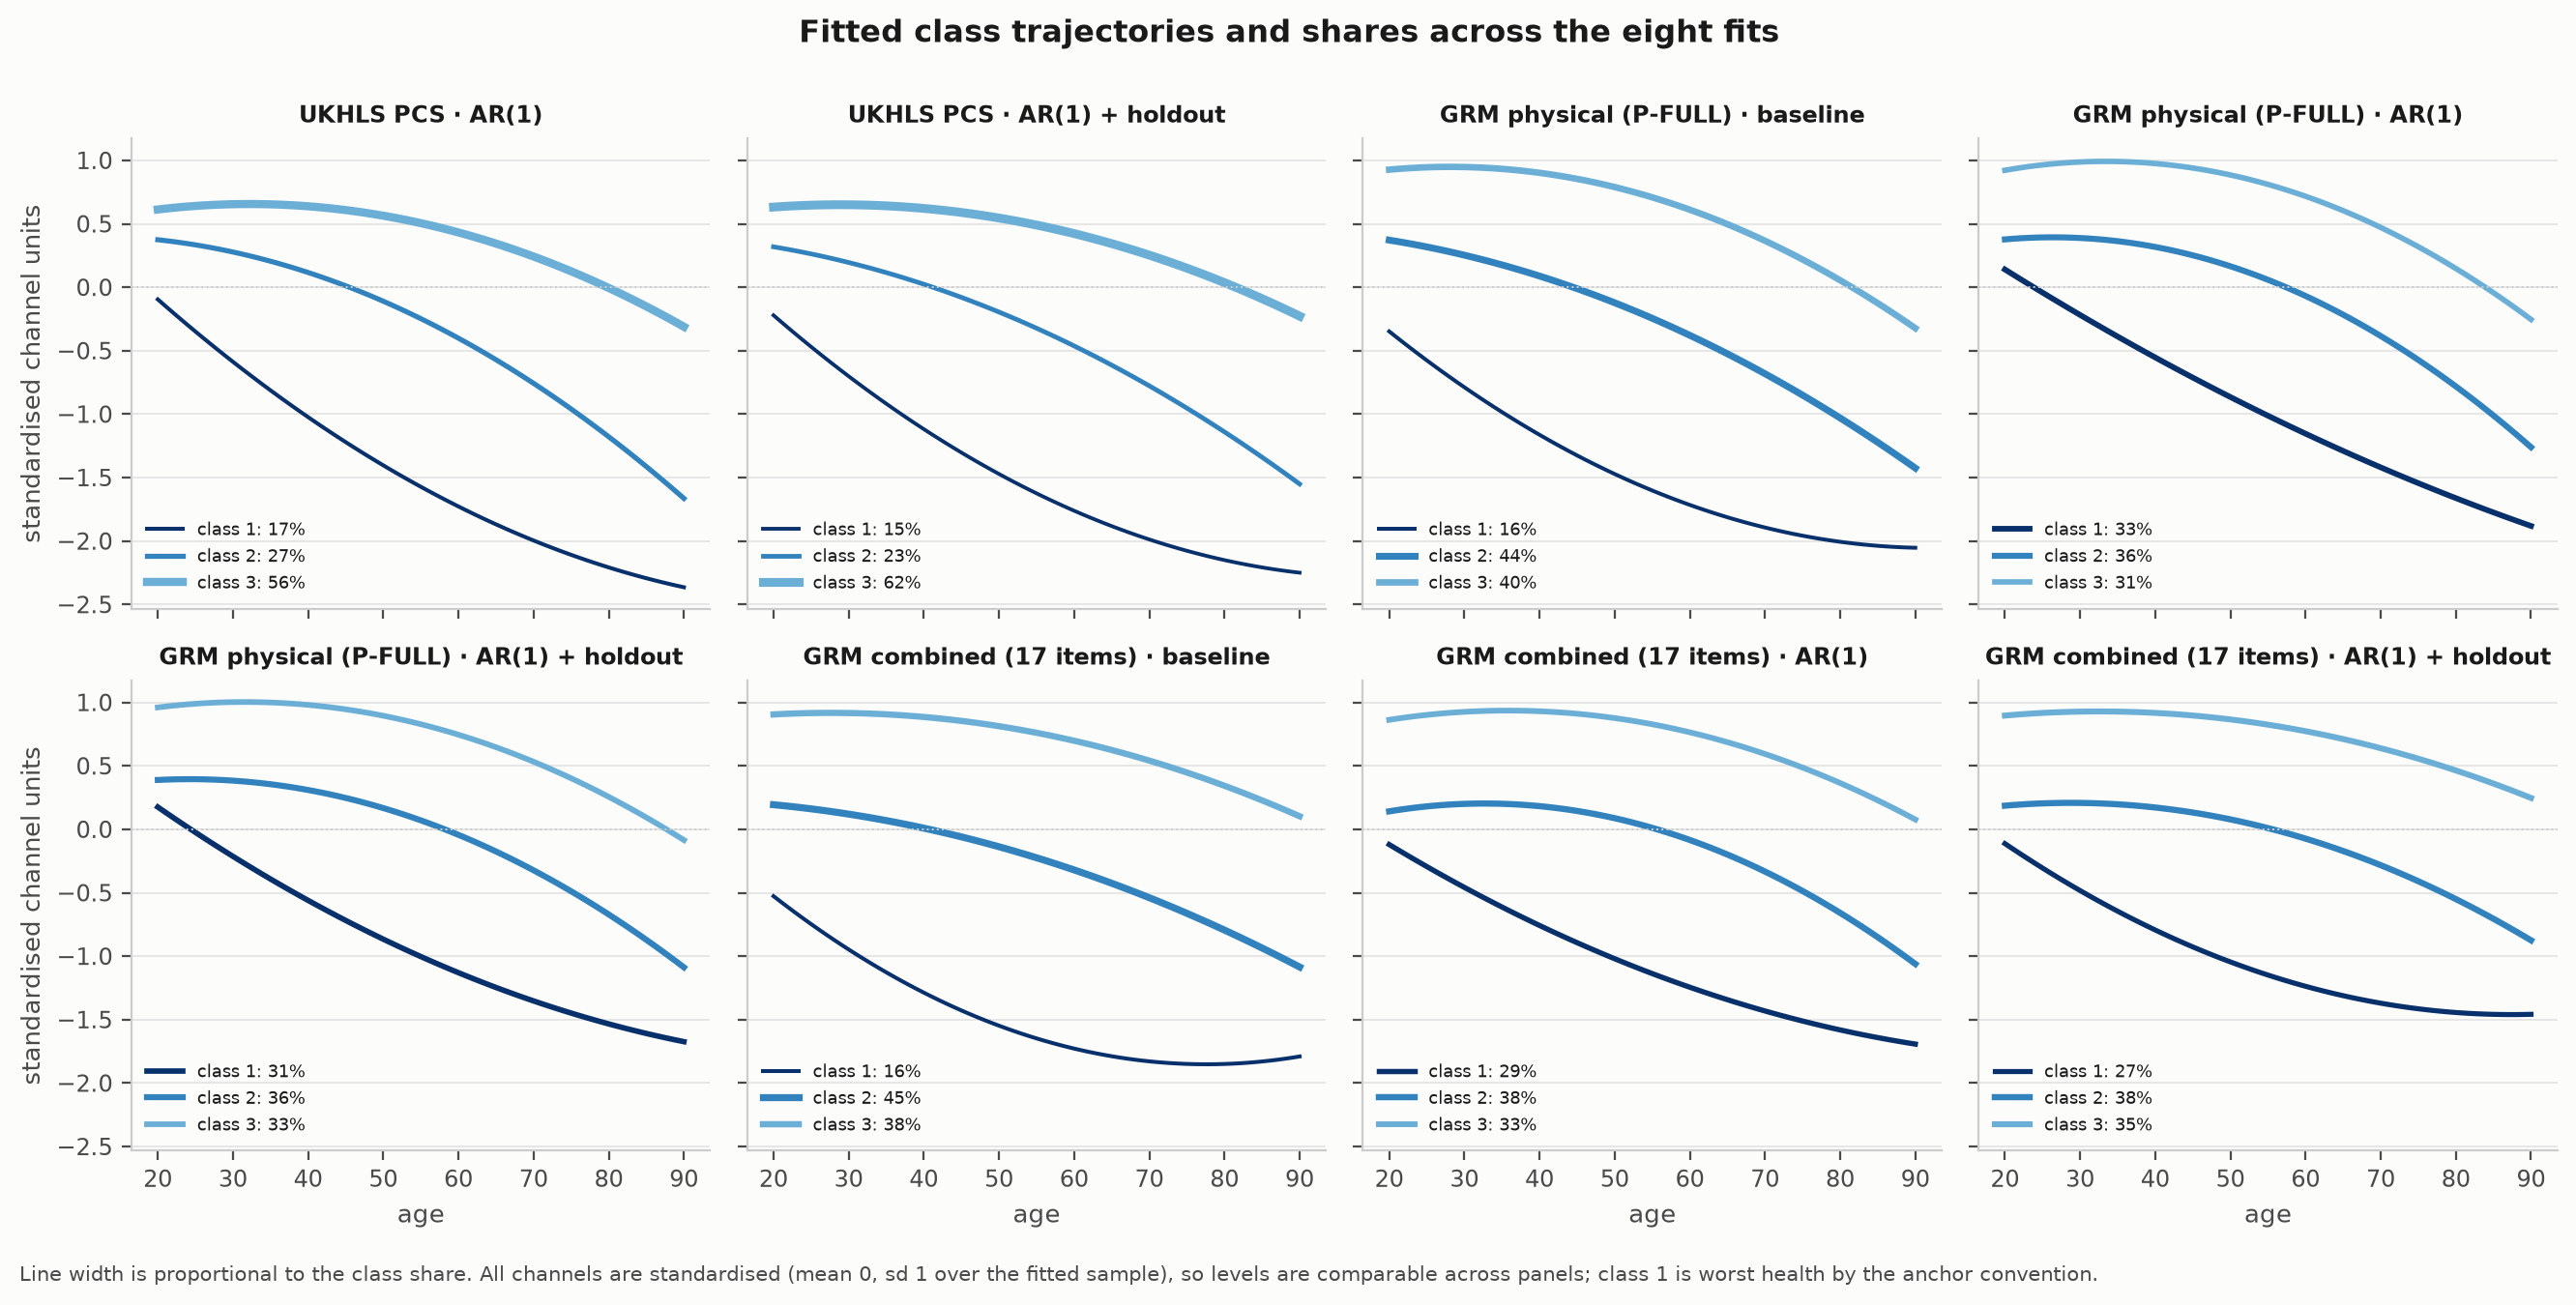
\includegraphics[width=\linewidth]{fig_trajectory_comparison}
\caption{Fitted class mean trajectories $\alpha_k + \beta_k a + \gamma_k
a^2$ (with $a = (\text{age}-55)/10$) for all eight fits, on each channel's
standardised scale. Channels: the UKHLS PCS, the physical GRM in its P-FULL
specification (\code{theta\_phys\_full}: functioning plus diagnosis groups),
and the combined seventeen-item GRM (\code{theta\_combined}). Line width is
proportional to the class share.}
\label{fig:trajectories}
\end{figure}

Figure~\ref{fig:trajectories} puts every fit on one standardised axis. Three
regularities hold everywhere: the three classes are ordered in level at
every age and never cross; all three decline; and the worst class declines
\emph{fastest}, so the classes fan apart over the life course. The gap
between the best and worst class widens from $1.2$--$1.9$ sd at age 30 to
$1.8$--$2.2$ sd at age 80.

\begin{center}\small
\begin{tabular}{lrrrrr}
\toprule
Fit & worst-class & \multicolumn{2}{c}{level gap (best $-$ worst)} &
\multicolumn{2}{c}{decline, age 30--80} \\
 & share & age 30 & age 80 & worst & best \\
\midrule
PCS, AR(1) & .165 & 1.24 & 2.20 & $-1.62$ & $-0.66$ \\
PCS, AR(1) + holdout & .146 & 1.35 & 2.19 & $-1.45$ & $-0.61$ \\
GRM phys, baseline & .159 & 1.74 & 2.06 & $-1.22$ & $-0.89$ \\
GRM phys, AR(1) & .328 & 1.21 & 1.81 & $-1.44$ & $-0.84$ \\
GRM phys, AR(1) + holdout & .313 & 1.22 & 1.79 & $-1.32$ & $-0.75$ \\
GRM comb, baseline & .163 & 1.86 & 2.19 & $-0.90$ & $-0.57$ \\
GRM comb, AR(1) & .290 & 1.38 & 1.95 & $-1.12$ & $-0.56$ \\
GRM comb, AR(1) + holdout & .271 & 1.41 & 1.91 & $-0.96$ & $-0.46$ \\
\bottomrule
\end{tabular}

{\scriptsize Standardised channel units. Class 1 is worst health.}
\end{center}

The specifications differ in \emph{how} they separate the classes, and the
difference is systematic. Adding the AR term to a GRM channel moves the
worst class up in level (its age-30 gap to the best class narrows from 1.74
to 1.21 on the physical channel) while making it decline more steeply
($-1.22 \to -1.44$) and roughly doubling its membership. In other words the
baseline finds a \emph{small, extreme, comparatively flat} worst class; with
persistence available the model instead finds a \emph{larger, less extreme,
faster-declining} one. The ratio of worst-class to best-class decline --- a
compact summary of how much of the story is trajectory divergence rather
than fixed level differences --- rises from $1.37$ to $1.72$ (physical) and
$1.57$ to $2.00$ (combined) when persistence is added, while the PCS sits
at $2.4$--$2.5$ in both its specifications.

The holdout fits track their full-sample siblings closely on every one of
these quantities (shares within $.02$, level gaps within $.11$ sd, declines
within $.18$ sd), so the restriction to people with five or more
observations changes the estimated typology very little.

\subsection*{Out-of-sample prediction}

\textbf{What the model's held-out density conditions on.} As the eight fits
were run, the Stan generated quantities restarted the AR(1) recursion at the
first held-out row with the \emph{stationary} variance, so the person's own
last fitted value was not carried forward through $\rho$. The fitted rows reach the held-out
rows only through the class posterior (the second held-out row does condition
on the first). That is a coherent estimand --- what the latent class
structure alone predicts --- but it is not the forecast a persistence model
is capable of, and it understates what these fits know. The model has since
been corrected (\S\ref{sec:gqfix}); the results below were computed offline
on the same rows, with the offline machinery first validated by reproducing
the fits' own stored held-out densities to a correlation of $0.9999998$. The
AR-conditional forecast uses the same class posterior but carries the last
fitted deviation forward, $\mu_k(a_h) + \rho_k^{G}\,(y_{\text{last}} -
\mu_k(a_{\text{last}}))$, with the gap-adjusted predictive variance.

Two benchmarks are estimated on the fitted rows only: an age-quadratic
Gaussian, and last-observation-carried-forward (LOCF), which is a strong
naive predictor for a persistent quantity like health.

\begin{center}\small
\begin{tabular}{llrrrrr}
\toprule
Channel & Predictor & LPD/obs & RMSE & $R^2$ & cover$_{50}$ & cover$_{90}$ \\
\midrule
PCS & model, AR-conditional & $\mathbf{-1.005}$ & 0.671 & $\mathbf{.614}$ & .56 & .89 \\
 & model, class-only (Stan) & $-1.043$ & 0.706 & .573 & .60 & .90 \\
 & LOCF & $-1.118$ & 0.740 & .531 & .61 & .90 \\
 & age-quadratic & $-1.416$ & 0.991 & .159 & .52 & .88 \\
\addlinespace
GRM phys & model, AR-conditional & $\mathbf{-0.889}$ & 0.589 & $\mathbf{.672}$ & .54 & .91 \\
 & model, class-only (Stan) & $-1.015$ & 0.665 & .582 & .53 & .91 \\
 & LOCF & $-0.994$ & 0.653 & .596 & .56 & .90 \\
 & age-quadratic & $-1.376$ & 0.958 & .133 & .50 & .90 \\
\addlinespace
GRM comb & model, AR-conditional & $\mathbf{-0.961}$ & 0.635 & $\mathbf{.627}$ & .54 & .90 \\
 & model, class-only (Stan) & $-1.079$ & 0.709 & .535 & .54 & .90 \\
 & LOCF & $-1.058$ & 0.697 & .551 & .56 & .90 \\
 & age-quadratic & $-1.452$ & 1.030 & .020 & .48 & .89 \\
\bottomrule
\end{tabular}

{\scriptsize Per held-out observation (two per person; 58--79k rows), on the
standardised channel scale. 400 posterior draws. cover$_{50}$ and
cover$_{90}$ are the empirical coverage of central predictive intervals
with nominal 0.50 and 0.90.}
\end{center}

\textbf{Age alone predicts almost nothing at the person level.} The
age-quadratic benchmark reaches $R^2 = .02$--$.16$. Everything interesting
in these data is between-person, which is the premise of the whole exercise
and is worth having measured.

\textbf{The class structure alone does not beat carrying the last
observation forward.} On the model's own estimand, the mixture edges LOCF on
the PCS ($R^2$ .573 vs .531) but \emph{loses} to it on both GRM channels
(.582 vs .596; .535 vs .551). A three-class typology plus an age polynomial
is roughly as informative about a person's next two observations as simply
assuming they will be where they were last time --- no better on the sharper
measures. Stated plainly: the classes describe lifecycle shape well, but
they are a coarse summary of an individual's current position.

\textbf{Persistence is what makes the model predict.} Carrying the last
deviation forward lifts $R^2$ to .61--.67, clearly ahead of LOCF on every
channel, and improves the log density by $.04$--$.13$ nats per observation.
The gain over LOCF is largest on the physical GRM (.672 vs .596). The two
ingredients are complementary: the class trajectory supplies where the
person is heading, $\rho$ supplies how much of where they are now to carry
with them, and LOCF is the degenerate case that keeps the level and ignores
the trajectory.

\textbf{The physical GRM predicts best on every metric} (LPD $-0.889$, RMSE
$0.589$, $R^2$ $.672$), ahead of the combined bank ($.627$) and the PCS
($.614$). This is the floor analysis (\S\ref{sec:ceiling}) showing up in
out-of-sample terms: a measure that resolves the ill tail finely gives the
model more to predict \emph{with} as well as more to predict.

\textbf{Calibration is good at the tails, mildly conservative in the
middle.} 90\% intervals cover 88--91\%, close to nominal. 50\% intervals
cover 48--61\%, over-covering on most fits --- and the same pattern appears
for the naive benchmarks, so it reflects health changes being more sharply
peaked than Gaussian rather than a defect of the mixture. A heavier-tailed
observation model (Student-$t$ residuals) is the natural refinement.

\subsection*{The corrected generated quantities}
\label{sec:gqfix}

The measurement above is a defect worth fixing rather than documenting, so
\code{person\_class\_loglik} now takes a \code{prev\_row} argument that
anchors the AR(1) recursion: $0$ opens a window at the stationary variance
(correct for a person's first fitted row), a row index opens it by carrying
that row's deviation forward. The generated-quantities block emits both
estimands rather than replacing one with the other ---
\code{log\_lik\_heldout} is now AR-conditional, and
\code{log\_lik\_heldout\_marginal} preserves the class-only quantity these
eight fits reported.

The model block is untouched: it passes \code{prev\_row = 0}, and
\code{log\_prob} at a fixed parameter point returns bit-identical values
before and after the change ($-15686.1620000000$ on the test payload). The
existing posteriors therefore remain valid --- only the reported held-out
quantity changes. \code{tests/test\_gq\_heldout.py} recomputes both
estimands in numpy from the same payload and draws and requires agreement to
$10^{-5}$, and checks that they coincide exactly when \code{ar\_mode == 0}.

What the corrected block reports on these fits, per held-out observation
(the joint density of the two-row window, so the second row conditions on
the first's realised value --- which is why it exceeds the row-by-row
forecast in the table above):

\begin{center}\small
\begin{tabular}{lrrr}
\toprule
Channel & class-only (as run) & AR-conditional (corrected) & gain \\
\midrule
PCS & $-1.043$ & $-0.964$ & $+0.079$ \\
GRM physical & $-1.015$ & $-0.836$ & $+0.180$ \\
GRM combined & $-1.079$ & $-0.908$ & $+0.171$ \\
\bottomrule
\end{tabular}
\end{center}

So the correction is worth $0.08$--$0.18$ nats per held-out observation on
the reported density, and most on the physical GRM --- the channel whose
persistence estimate is the strongest. Held-out numbers from the eight fits
in this note are the class-only column, and should be read as
class-structure diagnostics; anything refitted from here reports the
corrected quantity.

\textbf{Caveats.} The holdout samples are people with at least five
observations, who are healthier and better-retained than the full roster;
the holdout fits reproduce their full-sample siblings' structure closely
($\theta$ within .02, $\rho$ within .02 on every channel), which is
reassuring but does not make them representative. And the combined-channel
fits inherit \S\ref{sec:combined}'s unidimensionality caveat: a single class
structure over two correlated dimensions.

\subsection{How much of that convexity is real?}
\label{sec:convexdetail}

The figure above plots utilisation against \emph{percentiles} of each
measure, and the claim of convexity deserves more scrutiny than a percentile
axis can give it. Two separate things inflate it.

\textbf{The horizontal scale.} Percentiles are a rank transform, so equal
horizontal steps are equal shares of people rather than equal amounts of
health. For a roughly normal $\theta$ the bottom decile spans far more of the
health scale than the fifth does, and compressing it to the same width bends
the left-hand end upward. Panels (a) and (b) of
Figure~\ref{fig:convexdetail} show the same relationship on the two axes:
the sharp elbow on the percentile axis becomes a smooth decay on $\theta$.
The binning rule itself turns out not to matter --- equal-count and
equal-width bins trace the same curve --- so this is the axis, not the
aggregation. The formal test in the table above was already run on the
measure's own scale, so only the picture was affected; but the picture is
what carried the claim.

\textbf{The vertical scale, which matters more.} In-patient stays run at
$8.2\%$, and the logistic curve is convex everywhere below one half. A
relationship that is exactly \emph{linear in the log-odds} therefore appears
convex when plotted as a probability. Panel (b) draws a logistic with no
quadratic term at all against the observed decile means: it reproduces the
curvature almost exactly. Panel (c) puts the same data on the log-odds scale,
where it is close to a straight line.

\begin{figure}[H]
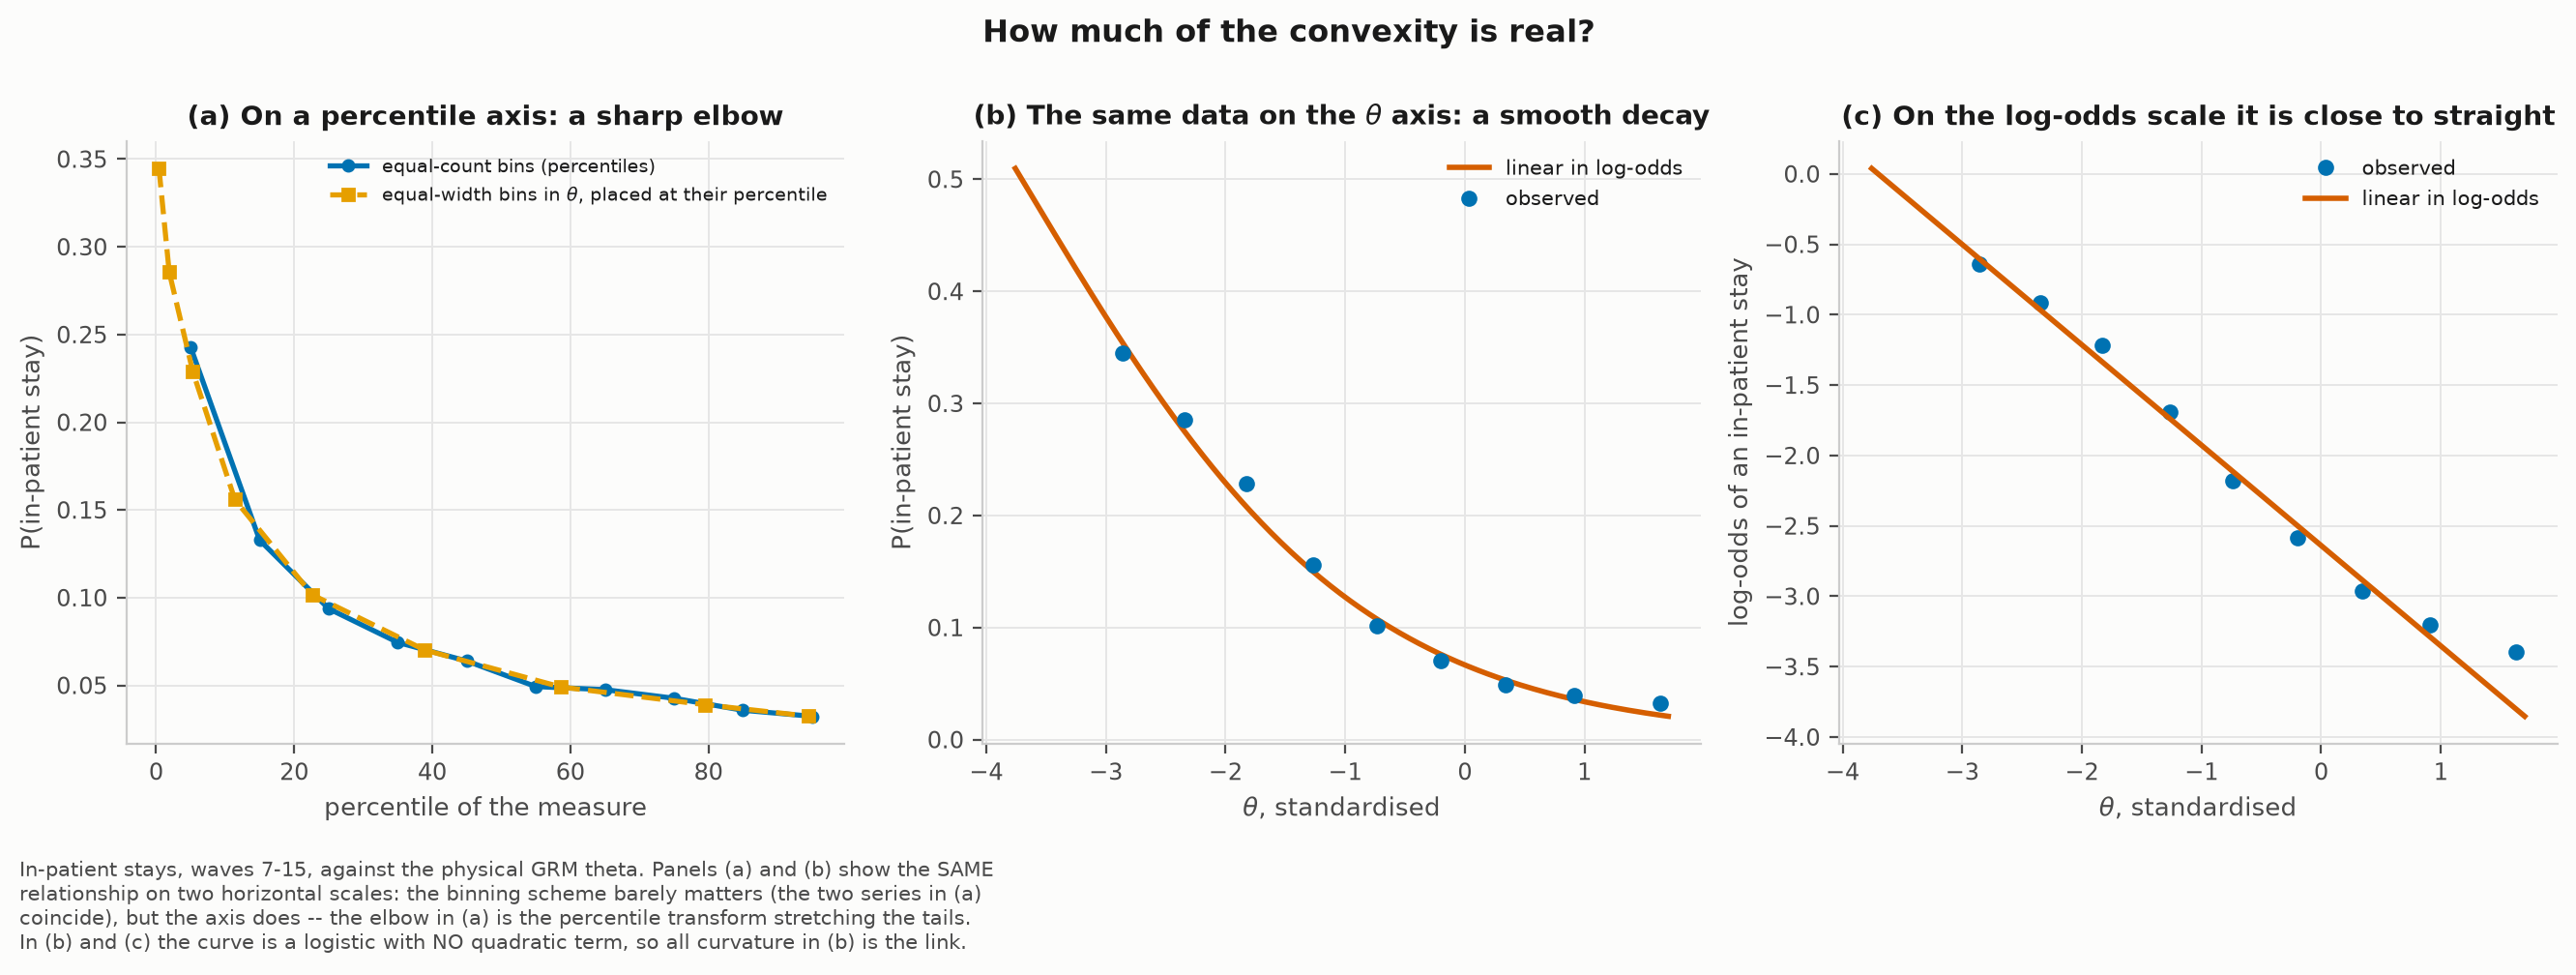
\includegraphics[width=\linewidth]{fig_convexity_detail}
\caption{In-patient stays against the physical GRM $\theta$. The fitted curve
in (b) and (c) is a logistic with no quadratic term, so every departure from
a straight line in (b) comes from the link function alone.}
\label{fig:convexdetail}
\end{figure}

Re-running the quadratic test on both scales makes the point numerically:

\begin{center}\small
\begin{tabular}{lrrrr}
\toprule
 & \multicolumn{2}{c}{probability scale} & \multicolumn{2}{c}{log-odds scale} \\
Measure & $z^2$ coef & $t$ & $z^2$ coef & $t$ \\
\midrule
GRM physical, $\theta$ & $+.020$ & 44.7 & $+.051$ & 8.6 \\
SF-6D utility & $+.021$ & 39.8 & $+.112$ & 18.1 \\
UKHLS PCS & $+.011$ & 23.7 & $\mathbf{-.028}$ & $-4.8$ \\
GRM physical, TCC scale & $+.009$ & 17.4 & $\mathbf{-.056}$ & $-10.2$ \\
\bottomrule
\end{tabular}
\end{center}

\textbf{On the probability scale every measure is emphatically convex; on the
log-odds scale two of the four change sign.} The PCS and the TCC
cardinalisation are mildly \emph{concave} in log-odds. Only $\theta$ and the
SF-6D remain convex there, and $\theta$'s curvature is small against its
linear slope of $-0.71$ per standard deviation.

\textbf{What this means for the framework.} The framework asks whether the
return to preventing a unit of health loss is larger for the already-unwell,
which is a question about the second derivative of a structural relationship
--- and a second derivative is not invariant to how either axis is
cardinalised. Three choices have to be made explicit before the question has
an answer: the health scale ($\theta$, its TCC transform, and the PCS rank
people almost identically but disagree about curvature), the outcome scale
(probability, log-odds, or eventually cost), and, if cost is the target, the
fact that we observe utilisation counts rather than spend at all. The honest
summary of \S\ref{sec:convexity} is therefore narrower than it first
appeared: \emph{utilisation falls steeply with health among the unwell and
flattens among the healthy, and on the natural multiplicative scale for a
risk that relationship is close to log-linear.} A convexity claim strong
enough to carry a policy conclusion needs a cost outcome and a defended
cardinalisation, neither of which UKHLS supplies on its own.

\subsection{What the literature actually establishes}
\label{sec:convexlit}

Convexity of healthcare costs in health is widely assumed in prevention
arguments, so it is worth separating what is \emph{accepted}, what is
\emph{measured}, and what is actually \emph{known} about the functional form.
The three come apart.

\textbf{Firmly measured, and about the distribution rather than the shape.}
Spending is extremely concentrated: the top decile of spenders accounts for
more than half of total expenditure, and about a third of them are still in
the top decile a year later. This is robust and uncontroversial, but it is a
fact about the \emph{marginal distribution of spending}, not about the
derivative of cost with respect to health. A concentrated outcome is
consistent with many shapes, including a linear one applied to a skewed
health distribution.

\textbf{Firmly measured, and genuinely about shape --- but on the count
scale.} The multimorbidity literature reports a ``near-exponential''
relationship between the number of chronic conditions and cost, with
expenditure roughly doubling per additional condition and specific
combinations costing more than the sum of their parts (superadditivity).
Here the scale is defensible in a way ours is not: ``one more condition'' has
a meaning that ``one more standard deviation of $\theta$'' does not. But note
what the finding \emph{is}: exponential in the count is exactly linear in log
cost. The headline result of that literature is a multiplicative model, which
is the same shape \S\ref{sec:convexdetail} found in our data --- not evidence
of curvature beyond multiplicative.

\textbf{Assumed by the standard specification, and therefore weakly tested.}
The default model for healthcare costs in health economics is a GLM with a
log link (Manning \& Mullahy 2001; Jones 2010), under which covariates act
multiplicatively by construction. A log-link model is convex in levels
automatically, whatever the data say. So a large share of the empirical
literature cannot be evidence \emph{for} convexity in levels, because it
imposes it; the interesting question --- is there curvature on the log scale?
--- is rarely posed. We found none of the reviewed work testing convexity
against a continuous health measure as a functional-form question.

\textbf{A rival explanation for the shape.} The ``red herring'' literature
(Zweifel, Felder \& Meiers 1999, and the twenty-year reappraisals) argues
that costs track \emph{proximity to death} rather than age or health level,
with spending tripling in the final quarters of life. If most of the
steepness at the bottom of the health distribution is people close to death,
then the apparent convexity in health is partly a survival gradient wearing a
health costume --- which our data cannot separate, because \S\ref{sec:multifit}
left mortality out of the fitted models.

\textbf{And a caution about the policy inference.} Even granting convexity,
Rose's prevention paradox (1981, 1985) blocks the automatic move from ``the
return per person is highest at the bottom'' to ``target the bottom'': most
cases arise from the large moderate-risk middle rather than the small extreme
tail, so aggregate returns can favour population-wide action even when
individual returns are convex. Convexity in the individual return function
and optimality of targeting are different claims.

\textbf{Where this leaves us.} The proposition that costs rise steeply as
health deteriorates is well measured and not in doubt. The stronger
proposition the framework needs --- that the second derivative is positive on
a defended scale, so that a unit of prevention is worth more to the already
unwell --- is much less established than its ubiquity suggests: it is usually
assumed through a log link, demonstrated on a count scale where it amounts to
log-linearity, or inferred from concentration statistics that do not identify
a shape. Our own finding of near-log-linearity
(\S\ref{sec:convexdetail}) sits comfortably within the literature rather than
against it. Testing the framework's version of the claim needs a cost outcome
rather than utilisation counts, a health scale defended on grounds other than
convenience, and mortality in the model so that proximity to death is not
doing the work.

\section{Towards a multidimensional model}
\label{sec:multidim}

The predecessor's five-channel mixed model used PCS and MCS (Gaussian),
self-rated health (ordered logit), a chronic count (negative binomial) and an
ADL count (hurdle negative binomial). Everything in this note argues for a
different set, and the binding constraint is coverage.

\begin{center}\small
\begin{tabular}{lrrl}
\toprule
Candidate channel & person-waves & persons & limiting gate \\
\midrule
$\theta$ physical, P-FUNC & 497{,}423 & 84{,}679 & none (every wave) \\
$\theta$ mental, without DEPR & 489{,}278 & 81{,}729 & none (every wave) \\
$\theta$ mental, as fitted (with DEPR) & 379{,}462 & 67{,}017 & diagnosis inventory \\
$\theta$ physical, P-FULL & 387{,}599 & 69{,}958 & diagnosis inventory \\
chronic count & \multicolumn{2}{c}{$76\%$ of person-waves} & diagnosis inventory \\
ADL count & \multicolumn{2}{c}{4 waves ($\sim 8\%$)} & scheduled module \\
\bottomrule
\end{tabular}
\end{center}

\textbf{One weak item is costing a quarter of the sample.} The mental bank as
fitted includes ever-diagnosed depression, which inherits the BHPS exclusion
of \S\ref{sec:routing}. Dropping that single item --- one hurdle, $a =
0.93$, the weakest item in the bank bar the rare diagnoses --- recovers
109{,}816 person-waves and 14{,}712 people, a $22.4\%$ increase. Jointly
observing a physical and a mental channel then covers 484{,}832 person-waves
on 81{,}458 people (49{,}545 of them with three or more observations),
against 376{,}019 / 66{,}841 / 38{,}478 if either channel carries a
diagnosis item. That is a $29\%$ larger estimation sample for the loss of
almost no information.

\textbf{Recommended specification.} Three channels, and the ragged-channel
machinery already in \code{runner/mixed.py} handles them as they stand:

\begin{enumerate}\itemsep2pt
\item \textbf{$\theta$ physical (P-FUNC)}, Gaussian. Replaces PCS and,
because self-rated health enters as the GH item and functioning as FUNC, it
also absorbs the old model's separate self-rated-health channel and its ADL
channel --- the latter traded for \code{disdif}, which measures the same
construct in every wave rather than four.
\item \textbf{$\theta$ mental without DEPR}, Gaussian. Replaces MCS, without
the orthogonality artifact, and with GHQ-12 doing most of the work.
\item \textbf{Chronic condition count}, negative binomial, on the $76\%$ of
person-waves where the inventory exists. Kept as a channel rather than folded
into a measurement model, which is where \S\ref{sec:ever} concluded it
belongs: ``ever'' is the correct state variable for a diagnosis, its
accumulation is a process to be modelled rather than an artefact to be
corrected, and as a channel its missingness is explicit instead of silently
deleting people.
\end{enumerate}

Two properties of this design matter. First, the class structure is
identified off channels 1 and 2, which are observed for everyone in every
wave, so the BHPS members contribute to the typology even though channel 3 is
missing for them --- the opposite of the current arrangement, where they are
dropped outright. Second, the missingness in channel 3 is a survey-design
gate, not a health-related process: the excluded people are indistinguishable
on every health measure (\S\ref{sec:routing}), so treating it as ignorable
conditional on the observed channels is defensible in a way that ADL's
scheduled-module missingness also is, but that attrition would not be.

\textbf{What to leave out, and why.} Utilisation (\S\ref{sec:convexity}) is
an outcome for validating the measures, not a health dimension to be
clustered on. SF-6D is a mixed physical--mental utility
(\S\ref{sec:combined}) and would duplicate both channels at once. The
combined GRM is physically dominated (Figure~\ref{fig:combmodel}) and its
residuals say the data want two dimensions, not one. SWEMWBS, loneliness and
the ADL module all fail the every-wave rule.

\textbf{An extension worth considering later.} Channels 1 and 2 currently
compress each domain to a point estimate and then treat it as data, discarding
the posterior sd the GRM already computes (\S\ref{sec:ceiling}: $0.27$ near
the population mean, rising to $0.65$ at the extremes). Passing that through
as a known measurement-error variance per observation is a small change to
the Gaussian channels and would stop the model reading heteroskedastic
measurement noise as heterogeneity in health --- which, given the ceiling and
floor results, is concentrated exactly in the classes the model cares most
about.

\section{The multidimensional model}
\label{sec:multifit}

The specification of \S\ref{sec:multidim} was fitted in four variants ---
baseline, holdout, AR(1), AR(1)+holdout --- on one common sample of 38{,}268
people and 388{,}774 person-waves, so the four differ by specification alone.
Three channels: the physical GRM (P-FUNC) and the mental GRM without DEPR,
both Gaussian, and the chronic count as a negative binomial, masked on the
$24\%$ of rows with no diagnosis inventory. Mortality was toggled off for
this round. All four converged.

\begin{center}\small
\begin{tabular}{lrlllr}
\toprule
Variant & max $\hat R$ & $\theta$ (shares) & $\rho$ & chronic at 55 & wall \\
\midrule
baseline & 1.0032 & .189 / .377 / .434 & --- & 2.6 / 1.4 / 0.13 & 8.0 h \\
holdout & 1.0049 & .187 / .371 / .442 & --- & 2.6 / 1.4 / 0.14 & 6.8 h \\
AR(1) & 1.0014 & .190 / .398 / .413 & .73 / .61 / .60 & 2.9 / 1.1 / 0.01 & 19.0 h \\
AR(1) + holdout & 1.0023 & .195 / .389 / .416 & .72 / .58 / .58 & 2.9 / 1.1 / 0.01 & 18.2 h \\
\bottomrule
\end{tabular}

{\scriptsize ``chronic at 55'' is the implied mean condition count at age 55
for each class.}
\end{center}

\textbf{Extra channels stabilise the classes against the AR term.} In the
univariate fits of \S\ref{sec:ar1} adding persistence roughly doubled the
worst class (.16 $\to$ .33 on both GRM channels). Here the shares are flat
across all four variants at about .19 / .38 / .42. The mechanism in
\S\ref{sec:ar1} was that a single channel cannot separate a small extreme
class from the autocorrelation of repeated low observations, so once $\rho$
can absorb the latter the boundary moves; with three channels the class is
identified from agreement \emph{across} channels, and persistence no longer
competes for the same variation.

\textbf{Persistence is much less class-graded than the univariate fits
implied.} $\rho = .73 / .61 / .60$ here, against $.78 / .27 / .39$ for the
physical GRM alone. The worst class remains the most persistent, but the
other two are far more so once a second correlated channel is observed: a
shock that looks transient in one measure reads as persistent when two move
together. That is a warning about reading $\rho$ off a single channel.

\textbf{The classes absorb the overdispersion in the chronic count.} The
implied means at 55 --- $2.6 / 1.4 / 0.13$ conditions --- weight up to $1.08$
against an observed mean of $1.045$, so the mixture reproduces the marginal.
And \code{phi\_chronic} settles at $656$ (baseline) to $920$ (AR), which for
a negative binomial is effectively Poisson: after conditioning on class and
age there is almost no overdispersion left to model.

\begin{figure}[H]
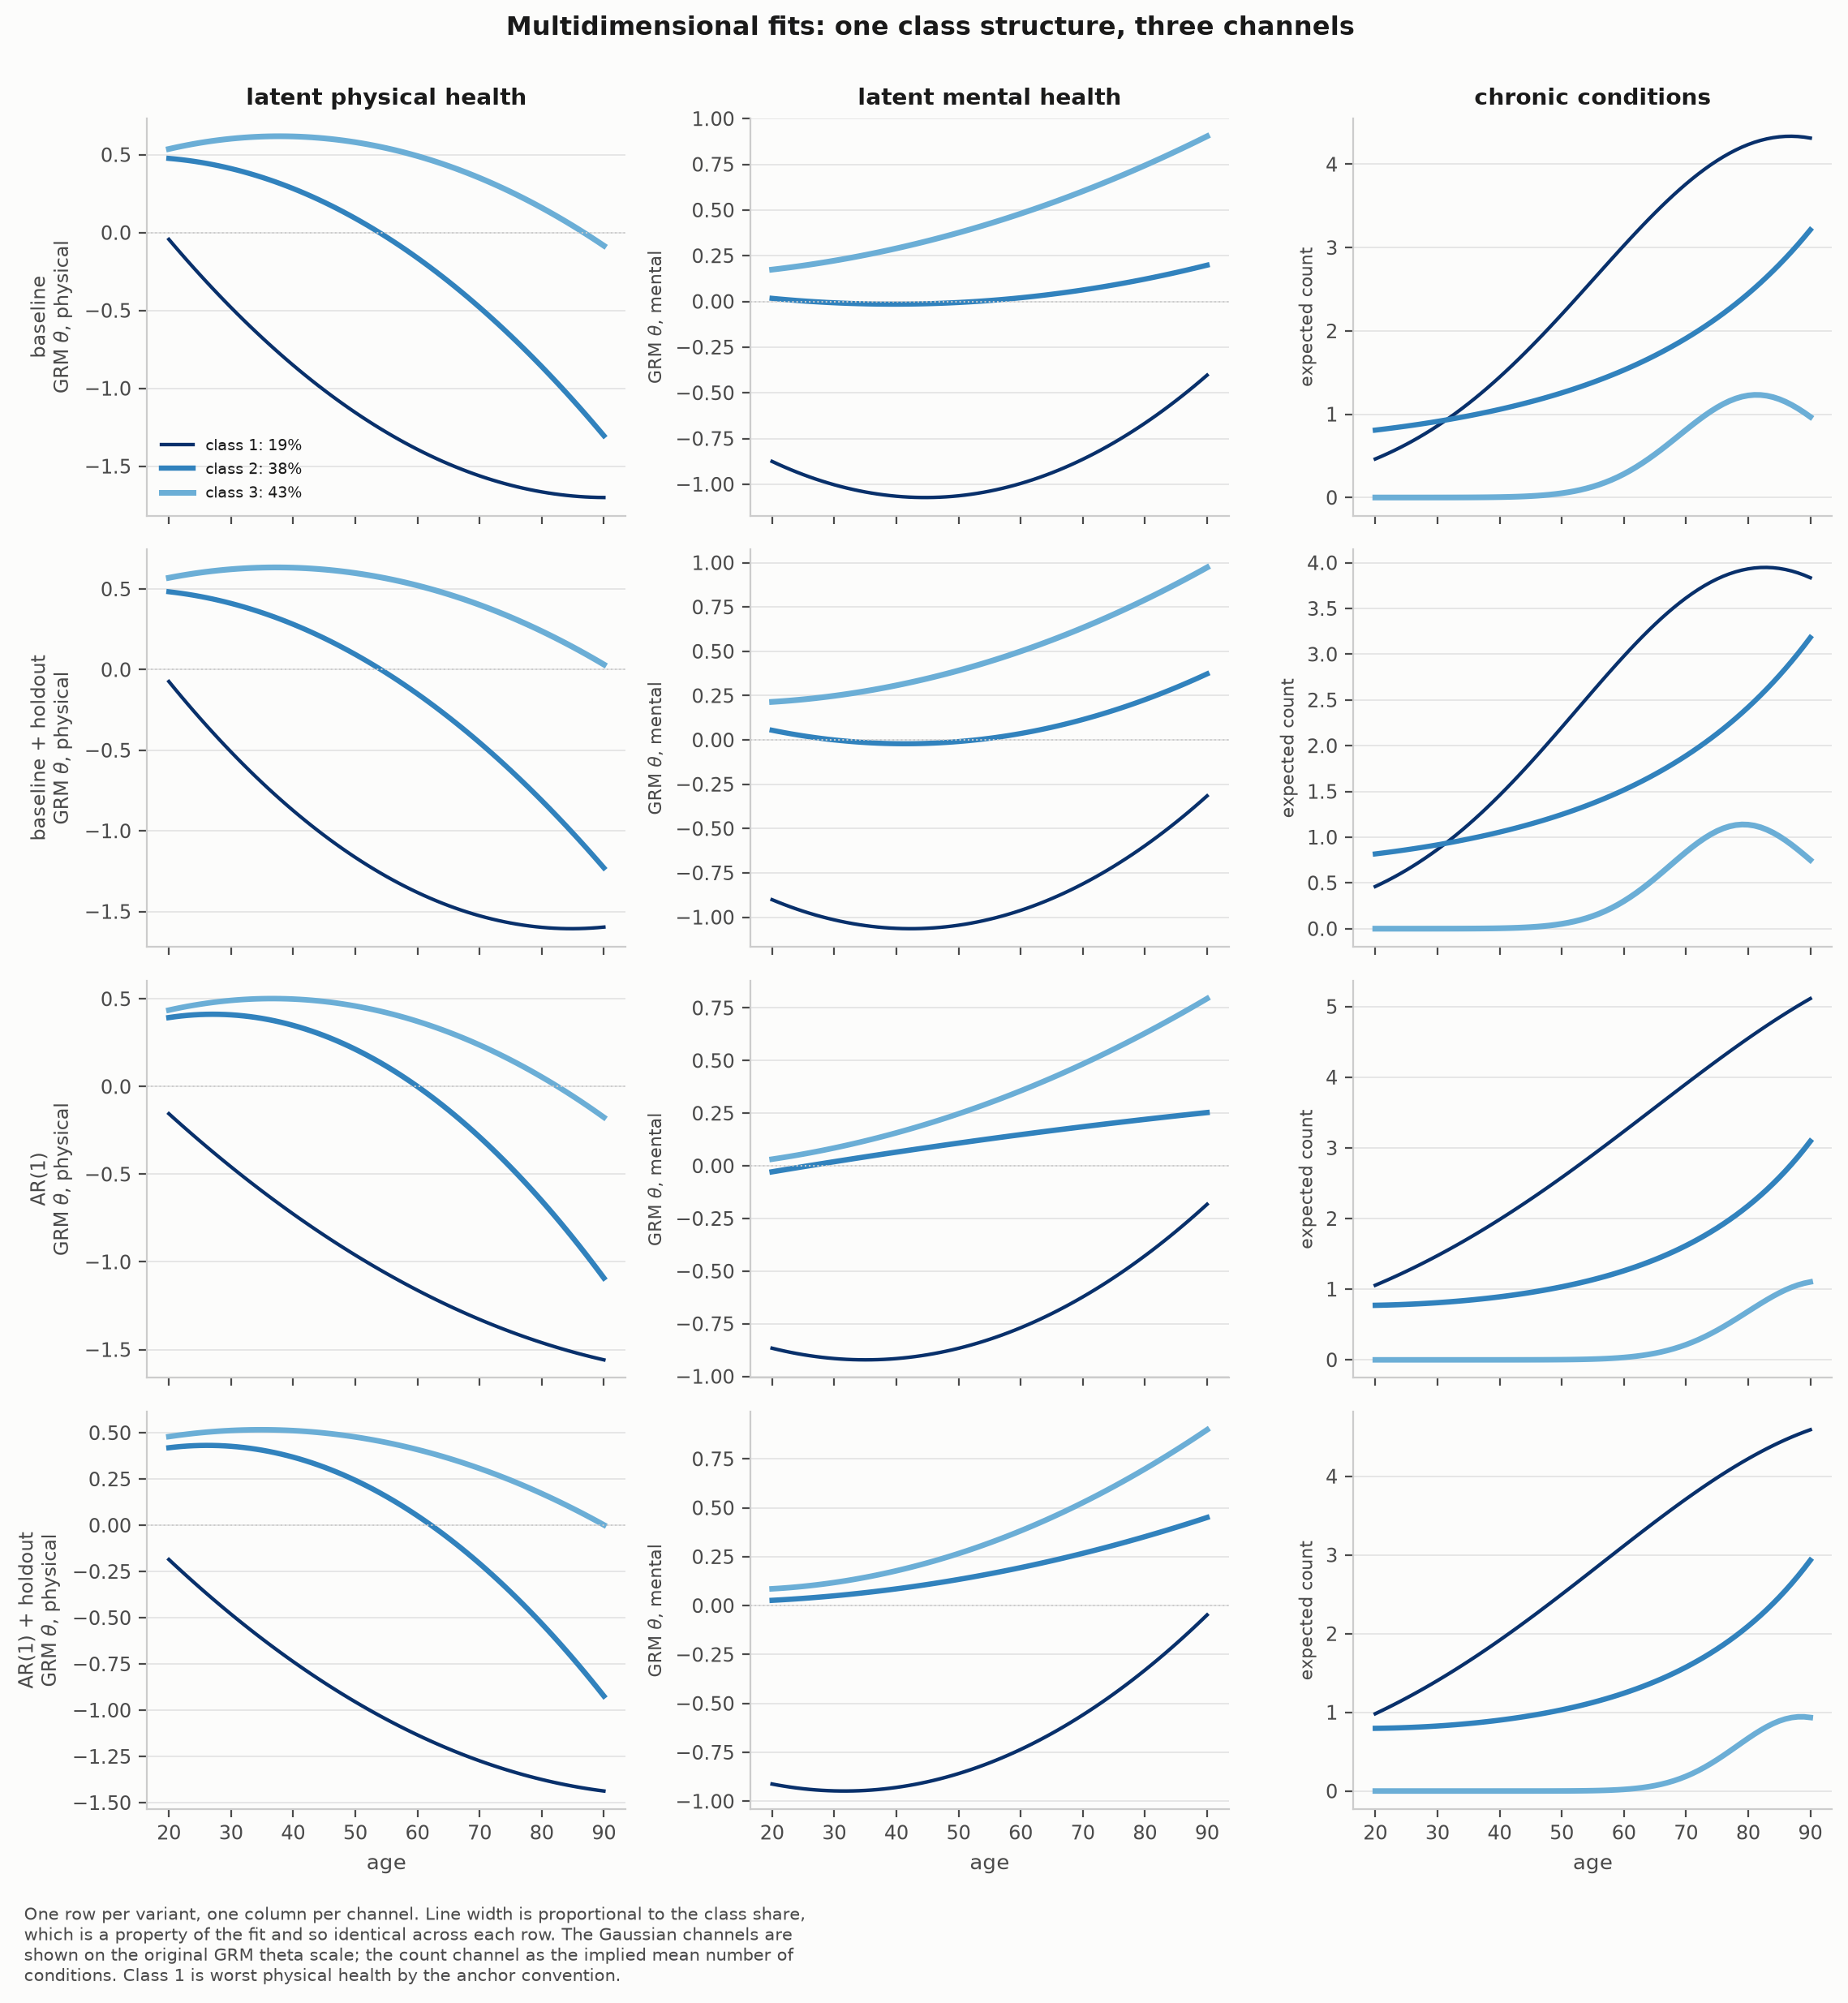
\includegraphics[width=\linewidth]{fig_multidim_trajectories}
\caption{Class trajectories and shares for the four multidimensional fits,
one row per variant and one column per channel. A fit has a single class
structure, so the shares are identical across a row and the line width
(proportional to the share) repeats; what changes across the row is what each
class \emph{does} on each channel. The Gaussian channels are returned to the
original GRM $\theta$ scale using each fit's standardising moments; the count
channel shows the implied mean number of conditions. Class 1 is worst
physical health by the anchor convention. Together with
Figure~\ref{fig:trajectories}, which covers the eight univariate fits, every
Bayesian model in this note has its trajectories and shares drawn.}
\label{fig:multitraj}
\end{figure}

Figure~\ref{fig:multitraj} makes the classes legible as types rather than as
parameter vectors. The physical channel behaves as the univariate fits led us
to expect: three ordered, non-crossing, accelerating declines, with class 1
falling from about $-0.1$ at age 20 to $-1.7$ at 90 while class 3 stays near
$+0.5$ until the sixties. The mental channel is where the multidimensional
model earns its keep. Its trajectories \emph{rise} with age for every class,
recovering the late-life wellbeing pattern of Figure~\ref{fig:moments} inside a
model that is simultaneously fitting a steep physical decline --- and they
rise fastest for class 3, so the healthiest physical type is also pulling
away mentally. Class 1 is worst on both channels at every age, which is worth
stating because nothing in the model forces it: only the physical channel
carries the ordering constraint, so the mental ordering is an estimate. The
count channel then separates the classes most sharply of the three, from
about $4.5$ conditions at age 80 in class 1 to $0.7$ in class 3.

The composition strips answer a question the shares alone cannot. In a
mixture $\theta$ is a lifetime constant, so any movement in a strip is
selection into the observed sample, not people changing class. Across the
twelve fits that movement is modest but consistent in sign for the physical
measures: the worst class rises from $12.1\%$ of person-waves at age 30 to
$18.8\%$ at 80 on the PCS, and from $29.8\%$ to $34.5\%$ on P-FULL under
AR(1) --- the healthiest are observed at every age while the least healthy
accumulate in the older cells. The multidimensional baselines tilt the other
way ($21.0\%$ at 30 falling to $15.3\%$ at 80), which is mortality and
attrition removing the sickest, and a reminder that these strips describe who
is present rather than how anyone's health evolved.

\subsection*{Held-out prediction, channel by channel}

Chronic is nearly free to predict --- carrying the last observed count
forward is exactly right on $93.4\%$ of the 58{,}600 held-out chronic rows
--- so a single held-out number would be flattered by it. The density is
therefore decomposed by channel offline, validated by reproducing the fits'
own stored per-person values (correlation $0.999999$, maximum deviation
$0.04$).

\begin{center}\small
\begin{tabular}{lrrr}
\toprule
 & \multicolumn{2}{c}{AR(1) + holdout} & holdout \\
Channel & AR-conditional & class-only & (no AR) \\
\midrule
$\theta$ physical & $-0.936$ & $-1.059$ & $-1.121$ \\
$\theta$ mental & $-1.138$ & $-1.245$ & $-1.321$ \\
chronic count & $-0.981$ & $-0.981$ & $-1.086$ \\
\midrule
all three & $-1.021$ & $-1.105$ & $-1.184$ \\
\bottomrule
\end{tabular}

{\scriptsize Log predictive density per held-out row. 76{,}536 rows on each
Gaussian channel, 58{,}623 on the count.}
\end{center}

Three readings. First, the two Gaussian channels gain $0.12$ and $0.11$ nats
per row from carrying the last value forward, while \textbf{the chronic
channel gains exactly zero} --- to three decimal places, because the model
carries no persistence term on that channel at all. It predicts the count
from class and age, never from the person's own previous count.

Second, that omission is expensive. The distribution of the change from a
person's last observed count is $93.4\%$ zero, $5.8\%$ $+1$, $0.6\%$ $+2$ or
more, with an entropy of $0.274$ nats. A channel that used the previous count
could therefore reach about $-0.27$ per row where the fitted model achieves
$-0.98$: roughly \textbf{0.7 nats per row left on the table}, far more than
the $0.12$ the AR term buys on the Gaussian side. This is the count-channel
analogue of the generated-quantities defect of \S\ref{sec:gqfix}, and the
obvious next fix: the chronic channel should condition on the last observed
count, either as an offset or through a monotone accumulation process.

Third, the physical channel predicts better than the mental one on every
variant ($-0.94$ against $-1.14$), the same ordering the univariate fits
found, and the non-AR holdout has AR-conditional and class-only densities
identical to four decimal places --- correct by construction when there is no
persistence to carry, and a useful check that the toggle behaves.

\textbf{Caveats.} Mortality is absent from this round, so nothing here speaks
to how the classes differ in survival. The GRM thetas enter as point
estimates: the posterior standard deviation the measurement model already
computes ($0.27$ near the population mean, $0.65$ at the extremes,
\S\ref{sec:ceiling}) is discarded, so the mixture reads heteroskedastic
measurement noise as heterogeneity in health, and does so most where the
extreme classes live. Passing that through as a known per-observation
variance is a small change to the Gaussian channels and the natural next
extension. Finally, the univariate comparison in \S\ref{sec:ar1} used P-FULL
while this model uses P-FUNC, so the two are not a nested pair; a univariate
P-FUNC fit would close that gap.

\section{Predicting outcomes the models never saw}
\label{sec:outcomes}

Everything so far scores a model against the health variables it was fitted
to. This section asks a different question: given a person's class posterior,
how well can we predict outcomes that appear in \emph{no} channel of
\emph{any} fitted model --- death, and healthcare use? Mortality was toggled
off for the multidimensional round and utilisation was never a channel, so
this is criterion validity, and it is the comparison that decides whether the
typology is useful beyond describing its own inputs.

Three outcomes: death during the panel (person-level), any in-patient stay in
the last twelve months, and the out-patient attendance band $0$--$4$ (both
person-wave, waves 7--15). Three predictor sets, each also carrying a
quadratic in age so that what is measured is what each adds to age alone:
age only; age plus the two free class posteriors; and age plus the model's
own continuous health measure, which is the fair competitor because it is
what the classes summarise. People are split $70/30$, the outcome model
fitted on the $70$ and scored on the $30$.

\begin{figure}[H]
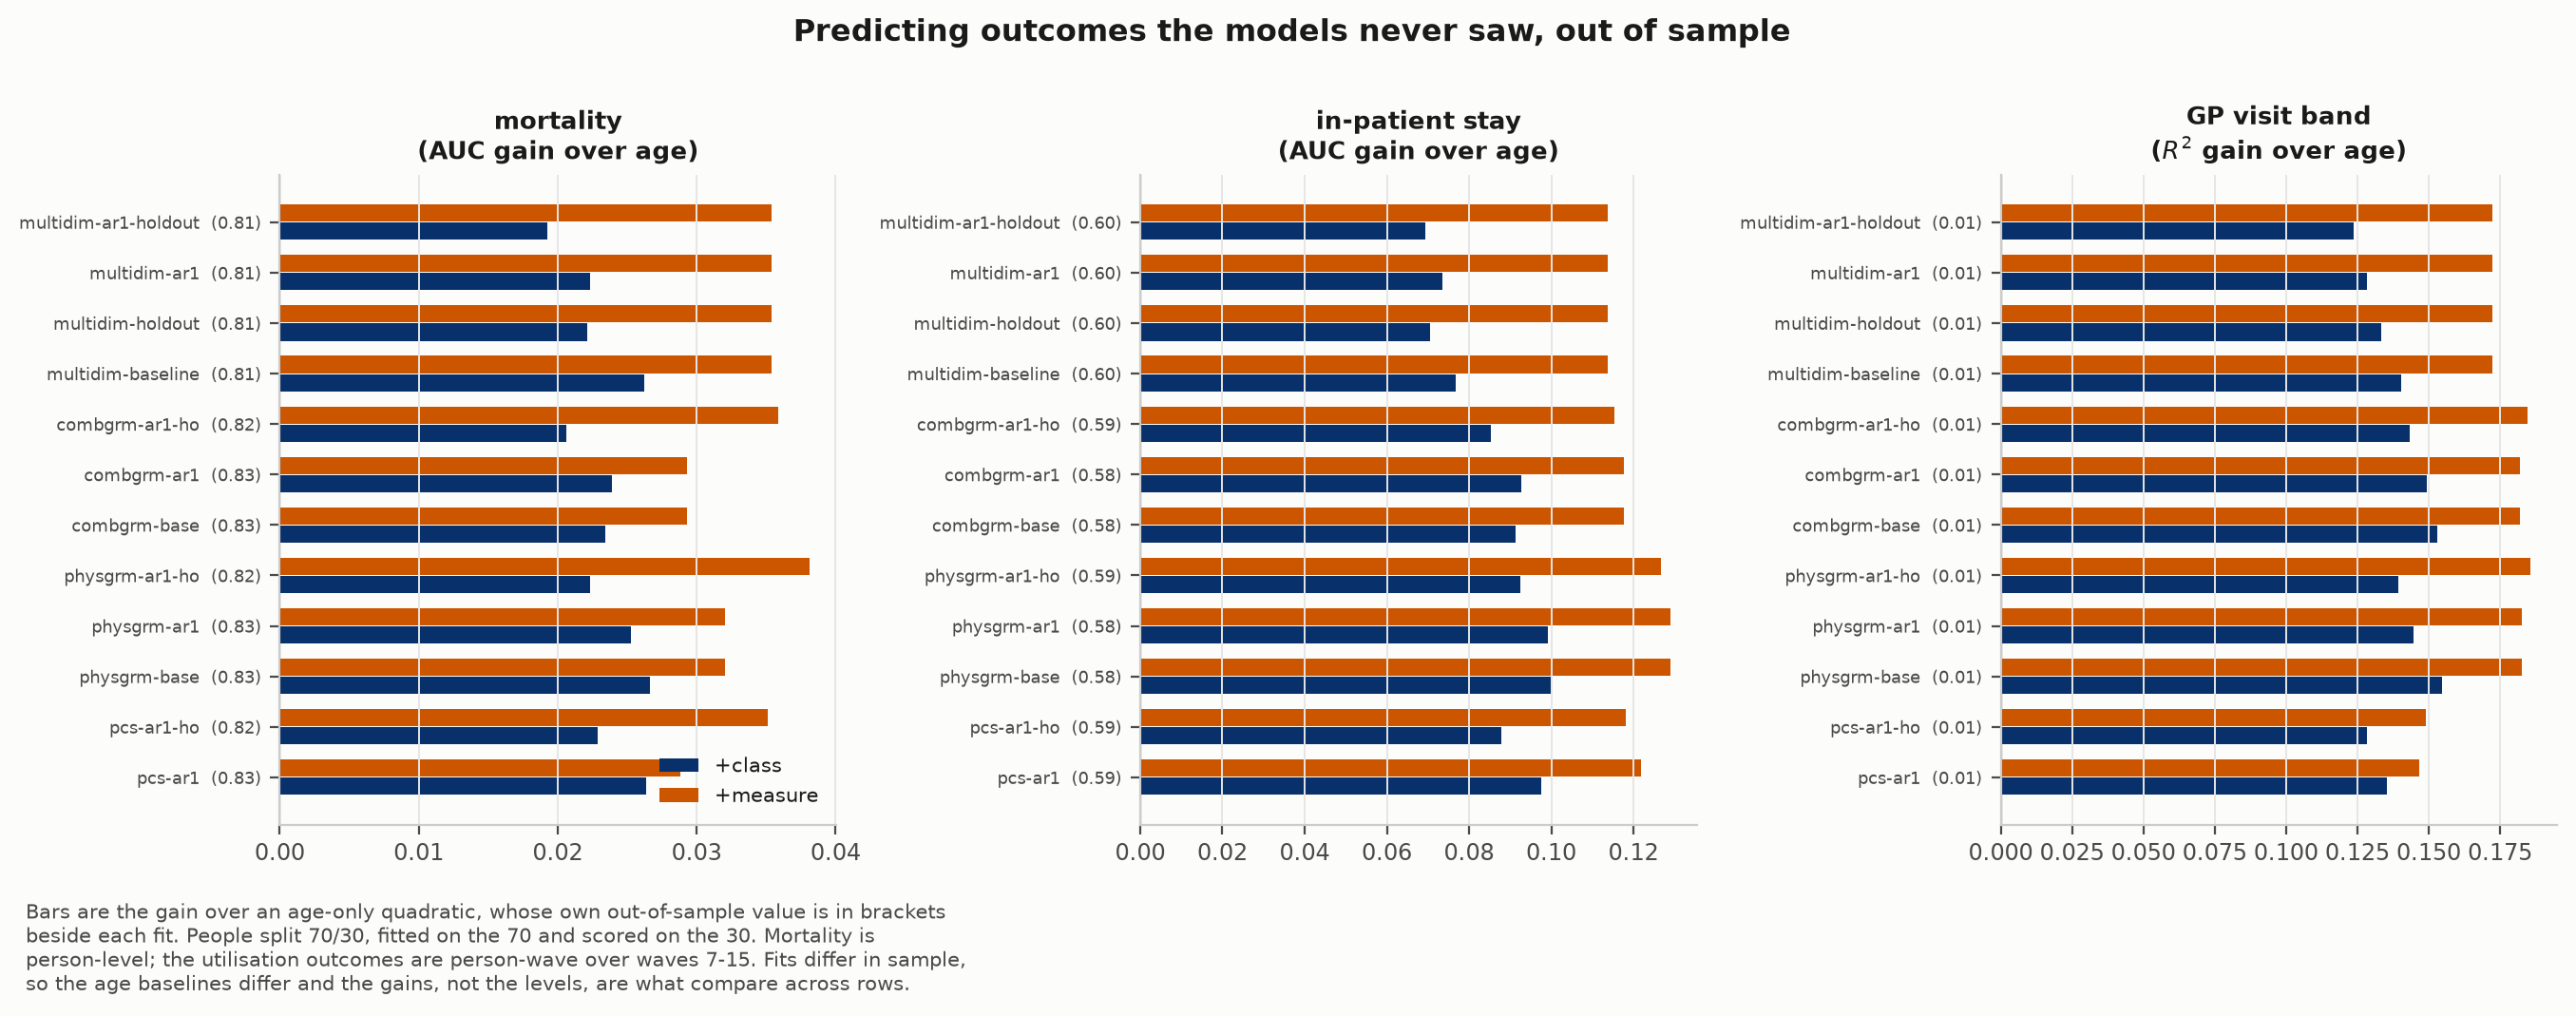
\includegraphics[width=\linewidth]{fig_outcome_prediction}
\caption{Out-of-sample gain over an age-only quadratic, whose own value is in
brackets beside each fit. Fits differ in sample, so the age baselines differ
and it is the gains, not the levels, that compare across rows.}
\label{fig:outcomes}
\end{figure}

\begin{center}\small
\begin{tabular}{lccc}
\toprule
 & mortality & in-patient & out-patient \\
 & \multicolumn{2}{c}{AUC, in / out} & $R^2$, in / out \\
\midrule
\multicolumn{4}{l}{\emph{age only}} \\
\quad PCS sample & .836 / .831 & .576 / .588 & .011 / .012 \\
\quad multidim sample & .828 / .815 & .586 / .596 & .010 / .012 \\
\addlinespace
\multicolumn{4}{l}{\emph{age + class posterior}} \\
\quad PCS, AR(1) & .856 / .857 & .678 / .686 & .143 / .148 \\
\quad P-FULL, baseline & .853 / \textbf{.861} & .674 / .681 & .155 / \textbf{.166} \\
\quad P-FULL, AR(1) & .852 / .860 & .675 / .680 & .148 / .157 \\
\quad combined, baseline & .850 / .856 & .664 / .672 & .157 / .165 \\
\quad multidim, baseline & .843 / .841 & .667 / .673 & .152 / .153 \\
\quad multidim, AR(1) & .841 / .837 & .663 / .670 & .144 / .141 \\
\addlinespace
\multicolumn{4}{l}{\emph{age + the continuous measure}} \\
\quad P-FULL & .860 / \textbf{.866} & .705 / \textbf{.710} & .187 / \textbf{.194} \\
\quad multidim (P-FUNC) & .855 / .850 & .705 / .710 & .182 / .185 \\
\bottomrule
\end{tabular}
\end{center}

\textbf{The continuous measure beats the classes on every outcome, in every
fit, in and out of sample.} For out-patient attendance the gap is large:
$R^2$ of $.194$ against $.166$, so discretising into three classes throws
away about a sixth of what the measure knows. For in-patient stays it is
$.710$ against $.681$ in AUC. This is the sharpest statement of a theme
running through the note --- the classes are a summary, and summarising
costs. If prediction is the goal, use $\theta$; the typology earns its place
by being interpretable and by describing trajectories, not by predicting
better than the thing it summarises.

\textbf{Age already predicts mortality well, and health adds little.} The
age-only AUC is $.83$, and the best class specification reaches $.861$ --- a
gain of about $.027$. Health measured in mid-life is a weak marginal
predictor of death once age is known, at least at this horizon. Utilisation
is the opposite: age alone gives AUC $.59$ for in-patient stays and
$R^2 = .01$ for out-patient bands, and health does the overwhelming majority
of the work. Prevention targeted on these measures should expect to move
utilisation far more readily than mortality.

\textbf{The multidimensional classes are not better than the univariate ones
at this, and are slightly worse.} On gain over age they are comparable for
mortality ($+.026$ against $+.027$ for P-FULL baseline) but behind on both
utilisation outcomes ($+.077$ against $+.100$ AUC for in-patient; $+.141$
against $+.154$ $R^2$ for out-patient). Adding channels bought stability and
interpretation (\S\ref{sec:multifit}), not external predictive power. Note
the samples differ, so only the gains are comparable, and the multidim
measure column is P-FUNC where the univariate is P-FULL.

\textbf{The AR variants predict external outcomes slightly worse than their
baselines}, consistently across all three outcomes and both families. That is
coherent with \S\ref{sec:ar1}: the AR term absorbs within-person variation
that would otherwise separate the classes, so the classes it leaves behind
carry marginally less information about anything else.

\textbf{Caveat.} The class posteriors come from mixtures fitted on all
people, so the $70/30$ split tests the class-to-outcome relationship out of
sample but not the whole pipeline; a fully clean version would refit each
mixture on the training people. In-sample and out-of-sample figures are
nonetheless close throughout --- often the out-of-sample number is the higher
of the two --- so there is little sign of the outcome models overfitting.

\section{Recommendations}

\begin{enumerate}\itemsep2pt
\item Physical health for lifecycle dynamics: \textbf{P-FUNC} (or the
original GRM). Mental health: \textbf{MENT}. Report both; their correlation
(0.457) is a finding, not an assumption.
\item \textbf{P-FULL} as the descriptive companion when condition burden
should show in the score; P-REC/P-TIMED quantify its recency sensitivity.
\item Conditions in the Bayesian mixture as separate channels; ``ever'' is
the right state variable there.
\item Avoid the combined score unless a single index is externally required;
if it is, build the bifactor version first.
\item SF-6D: treat as a mixed physical--mental utility (its closest GRM
cousin is the combined bank), never as a physical measure; licence before
publishing utilities.
\item Report $\theta$ and \code{grmh} together when consequences matter:
$\theta$ is the latent-normal unit the models want, \code{grmh} the
near-linear-in-utilisation unit (\S\ref{sec:convexity}); the choice of
cardinalisation is substantive, not cosmetic.
\end{enumerate}

\section{Reproducibility}

\begin{center}\small
\begin{tabular}{lp{6.4cm}}
\toprule
\code{data\_cleaning/03\_build\_measures.py} & SF-12/SF-6D layer; validates
against the construction note (max err 0.0054, 528{,}485 rows, the 6.6-pt
artifact, tariff checks) \\
\code{data\_cleaning/04\_build\_grm.py} & original GRM replicated to
$10^{-5}$ on all 498{,}424 person-waves \\
\code{data\_cleaning/05\_build\_chronic.py} & chronic layer; 100\% timing
coverage; $\ge$ EIT count on 100.000\% of rows \\
\code{data\_cleaning/06\_build\_grm2.py} & all GRM-2 specs; Q3, EAP
identity, invariance, recency weights \\
\code{descriptives/01--12} & measure panel, correlations, every figure, the
ceiling/floor, convexity, class-composition and outcome-prediction tables \\
\code{clustering/run\_fit.py}, \code{runs/overnight\_queue.py} & the
\S\ref{sec:ar1} batch: generic registry fits, last-two-observations holdout,
per-person held-out densities \\
\code{clustering/run\_multidim.py}, \code{runs/multidim\_queue.py},
\code{multidim\_channel\_decomp.py} & the \S\ref{sec:multifit} batch and its
per-channel held-out decomposition \\
\bottomrule
\end{tabular}
\end{center}

Everything under \code{data/} derives from licensed UKHLS microdata and is
never committed; all figures are aggregate statistics.

\subsection*{References}
{\small
Barnett et al.\ (2012) \emph{Lancet} 380:37--43.
Bauer \& Hussong (2009) \emph{Psychol Methods} 14:101--25.
Cella et al.\ (2010) \emph{J Clin Epidemiol} 63:1179--94.
Farivar, Cunningham \& Hays (2007) \emph{Health Qual Life Outcomes} 5:54.
Goldberg et al.\ (1997) \emph{Psychol Med} 27:191--7.
Graetz (1991) \emph{Soc Psychiatry Psychiatr Epidemiol} 26:132--8.
Hankins (2008) \emph{Clin Pract Epidemiol Ment Health} 4:10.
Johnston, Propper \& Shields (2009) \emph{J Health Econ} 28:540--52.
Jones (2010) \emph{Models for health care}, HEDG WP 10/01.
Kelly et al.\ (2024) \emph{Pharmacoepidemiol Drug Saf} 33:e5701.
Manning \& Mullahy (2001) \emph{J Health Econ} 20:461--94.
Kriegsman et al.\ (1996) \emph{J Clin Epidemiol} 49:1407--17.
Mitnitski, Mogilner \& Rockwood (2001) \emph{ScientificWorldJournal} 1:323--36.
Preen et al.\ (2006) \emph{J Clin Epidemiol} 59:940--6.
Samejima (1969) \emph{Psychometrika Monogr} 17.
Searle et al.\ (2008) \emph{BMC Geriatr} 8:24.
Sylvestre \& Abrahamowicz (2009) \emph{Stat Med} 28:3437--53.
Wainer \& Kiely (1987) \emph{J Educ Meas} 24:185--201.
Ware, Kosinski \& Keller (1996) \emph{Med Care} 34:220--33.
Yen (1993) \emph{J Educ Meas} 30:187--213.
Rose (1981) \emph{BMJ} 282:1847--51; (1985) \emph{Int J Epidemiol} 14:32--8.
Zweifel, Felder \& Meiers (1999) \emph{Health Econ} 8:485--96.
}

\end{document}
